\documentclass[a4paper,12pt,openany]{report}
\usepackage[utf8]{inputenc}  %pour utiliser les mots avec accents
\usepackage[T1]{fontenc}   % utiliser tous les caractères du clavier
\usepackage[french]{layout}  % pour paramétrer les marges du document
\usepackage{here}
\usepackage{latexsym}  %Pour utiliser divers symboles mathématiques
\usepackage{textcomp}
\usepackage{amsfonts}        %pour gerer le fond des couleurs
\usepackage{amssymb}         %POUR GERER LES FORMULES ET EXPRESSIONS MATHEMATIQUES
\usepackage{amsthm}         %POUR GERER LES FORMULES ET EXPRESSIONS MATHEMATIQUES
\usepackage{mathrsfs}
\usepackage[centertags]{amsmath}   %POUR GERER LES FORMULES ET EXPRESSIONS MATHEMATIQUES
\usepackage{fancyhdr}        %Pour personnaliser l'en-tête et pied de page
\usepackage[dvips]{epsfig}
\usepackage{color}     %pour colorer du texte dans le document
\usepackage{float}
\usepackage{times}
\usepackage{shadow} %pour gerer les ombres
\usepackage{txfonts}
%\usepackage[colorlinks, citecolor=blue]{hyperref}
\usepackage[french]{babel}
\usepackage{graphicx}    %Pour inserer des images
\usepackage{colortbl}
\usepackage{fancybox}           %Pour GERER LES BOX ET ENCADREMENTS
\usepackage{rotating}
\usepackage[left=2cm, right=2cm, top=2.5cm, bottom=2.5cm]{geometry} %POUR la taille des marges
\pagestyle{headings}
\usepackage{slashbox}       %Pour SCINDER LES CASES DU TABLEAU
\usepackage{framed}
\usepackage{sectsty}
\usepackage[french]{minitoc}
\usepackage{tabularx,cellspace}
\usepackage{diagbox}
\usepackage{setspace}            %Pour configurer l'interligne
\usepackage{boiboites}   %POUR configurer les encadrements des théorèmes
\usepackage{multicol}
\usepackage{bbold}     %POUR l'indicatrice
\usepackage{dsfont}
\newcommand{\fact}[1]{#1\mathpunct{}!}
\usepackage{listings}
\usepackage{color}
\usepackage{multirow}
\usepackage{siunitx}
\usepackage{tabularx} % Pour ajuster la largeur du tableau à la page
\usepackage{booktabs} % Pour de meilleures lignes dans les tableaux (toprule, midrule, bottomrule)
\usepackage{nomencl}
\usepackage{float} % Permet le placement strict des figures avec [H]
\usepackage{natbib}
% Définir une couleur verte claire personnalisée (optionnel, mais recommandé pour un dégradé)
\definecolor{lightgreen}{HTML}{C8E6C9} % Un vert très pâle, HEX code
% Ou une couleur prédéfinie de xcolor, par exemple : lightgray
\definecolor{mediumgreen}{HTML}{A5D6A7} 

% Définir les marges et la mise en page
%\usepackage[a4paper, total={18cm,25cm}]{geometry}

\definecolor{codegreen}{rgb}{0,0.6,0}
\definecolor{codegray}{rgb}{0.5,0.5,0.5}
\definecolor{codepurple}{rgb}{0.58,0,0.82}
\definecolor{backcolour}{rgb}{0.95,0.95,0.92}

\lstdefinestyle{mystyle}{
    backgroundcolor=\color{backcolour},
    commentstyle=\color{codegreen},
    keywordstyle=\color{magenta},
    numberstyle=\tiny\color{codegray},
    stringstyle=\color{codepurple},
    basicstyle=\footnotesize,
    breakatwhitespace=false,
    breaklines=true,
    captionpos=b,
    keepspaces=true,
    numbers=left,
    numbersep=5pt,
    showspaces=false,
    showstringspaces=false,
    showtabs=false,
    tabsize=2
}

\lstset{style=mystyle}



%COMMANDES pour personnaliser les dimensions du format et l'interligne %

\frenchspacing
\linespread{1.3}
\pagestyle{fancy}
\newcommand{\nocontentsline}[3]{}
\newcommand{\tocless}[2]{\bgroup\let\addcontentsline=\nocontentsline#1{#2}\egroup}





%COMMANDES pour personnaliser l'affichage des entêtes et pieds de pages 

%=================================================================================================================== %
\fancyhf{}

% Définit le pied de page droit (R pour Right, F pour Foot)
% \thepage est la commande LaTeX qui affiche le numéro de page actuel.
\fancyfoot[R]{\thepage}
%COMMANDES pour personnaliser l'affichage des entêtes et pieds de pages 
% Définition d'une couleur bleu clair
\definecolor{lightblue}{rgb}{0.8, 0.9, 1.0} 
\definecolor{vertclair}{rgb}{0.85, 0.95, 0.85}

\renewcommand{\sectionmark}[1]{\markright{\thesection\ #1}}
%\fancyhf{} \fancyfoot[c]{\bfseries\thepage}
%\fancyhead[L]{\bfseries\rightmark} \fancyhead[R]{\bfseries\leftmark}

% Thème dans un box avec fond bleu clair, au centre de l'entête
\fancyhead[C]{%
    \fcolorbox{black}{vertclair}{% % fcolorbox{cadre_couleur}{fond_couleur}{contenu}
        \parbox{\dimexpr\textwidth-2\fboxsep-2\fboxrule}{% % Calcule la largeur de la parbox pour qu'elle s'adapte à la largeur du texte
            \centering\bfseries\small MODÉLISATION PRÉDICTIVE DES CONDITIONS MÉTÉOROLOGIQUES AUX PORT AUTONOME DE DOUALA À PARTIR DE L'IA%
        }%
    }%
}

\renewcommand{\headrulewidth}{2pt}
\addtolength{\headheight}{0.5pt}
\renewcommand{\footrulewidth}{2pt}
\fancypagestyle{plain}{ \fancyhead{} \renewcommand{\headrulewidth}{0pt} }
%\newcommand{\clearemptydoublepage}{\newpage{\pagestyle{plain}\cleardoublepage}}
%\rhead{\textbf{\thepage}}
%\rfoot{\textbf{UNUVERSITE DE DOUALA}}
%\rfoot{\textbf{MÉMOIRE DE FIN D'ÉTUDE 2024-2025}} 
\lfoot{Mémoire De Fin D'étude D'ingénieur En Météorologie De L'ENSPD-UDO  \\\textit{Rédigé et présenté par} : \textbf{ENGOULOU SIKANDI Thierry}}

\newlength{\defbaselineskip}
\setlength{\defbaselineskip}{\baselineskip}
\newcommand{\setlinespacing}[1]{\setlength{\baselineskip}{#1 \defbaselineskip}}
\fancyfoot[r]{\fcolorbox{gray}{mhd}{\color{white}\textbf{\thepage}}  }

%========================================================================================================== %



%\renewcommand{\sectionmark}[1]{\markright{\thesection\ #1}}
%\fancyhf{} \fancyfoot[c]{\bfseries\thepage}
%\fancyhead[L]{\bfseries\rightmark} \fancyhead[R]{\bfseries\leftmark}
%\renewcommand{\headrulewidth}{2pt}
%\addtolength{\headheight}{0.5pt}
%\renewcommand{\footrulewidth}{2pt}
%\fancypagestyle{plain}{ \fancyhead{} \renewcommand{\headrulewidth}{0pt} }
%\newcommand{\clearemptydoublepage}{\newpage{\pagestyle{plain}\cleardoublepage}}
%\rhead{\textbf{\thepage}}
%\rfoot{\textbf{UNUVERSITE DE DOUALA}}
%\rfoot{\textbf{MÉMOIRE DE FIN D'ÉTUDE 2024-2025}} 
%\lfoot{\textbf{ENSPD}}
%
%\newlength{\defbaselineskip}
%\setlength{\defbaselineskip}{\baselineskip}
%\newcommand{\setlinespacing}[1]{\setlength{\baselineskip}{#1 \defbaselineskip}}
%\fancyfoot[c]{\fcolorbox{gray}{black}{\color{white}\textbf{\thepage}}  }






% % % %  Made by The_Solver   % % % % % % %

%COMMANDES pour personnaliser l'affichage des titres des chapitres 

\makeatletter 
\newcommand{\thechapterwords}
{ \ifcase \thechapter\or Un\or Deux\or Trois\or Quatre\fi}
\def\thickhrulefill{\leavevmode \leaders \hrule height 1ex \hfill \kern \z@}
\def\@makechapterhead#1{\vspace*{15\p@}  {\parindent \z@ \centering \reset@font
		\thickhrulefill\quad
		\quad  \fcolorbox{gray}{mhd}{\color{white}\textbf{ \@chapapp{} \thechapterwords}} 
		%bleu=couleur_bordure_du cadre  
		%rouge=couleur_à_l'intérieur_du_box  
		%blanc=couleur_du titre_chapitre 		
		\quad \thickhrulefill \par\nobreak \vspace*{15\p@} \interlinepenalty\@M \hrule
		\vspace*{15\p@} \Large \bfseries #1\par\nobreak \par \vspace*{15\p@} \hrule \vskip 60\p@ }}



%COMMANDES pour peronnaliser l'affichage de la table des matières %	

\def\@makeschapterhead#1{\vspace*{15\p@}  {\parindent \z@ \centering \reset@font \thickhrulefill
		\par\nobreak \vspace*{15\p@} \interlinepenalty\@M \hrule \vspace*{15\p@} \Huge \bfseries #1\par\nobreak
		\par \vspace*{15\p@} \hrule \vskip 60\p@ }}	


%LES COULEURS utilisées pour mon mémoire  


\definecolor{th}{rgb}{0.1,0.8,0.7}
\definecolor{vrt1}{rgb}{0.03, 0.29, 0.14}
\definecolor{vrt2}{rgb}{0.00, 0.39, 0.18}
\definecolor{gr1}{rgb}{0.68, 0.69, 0.70}
\definecolor{rg1}{rgb}{0.40, 0.14, 0.14}
\definecolor{vrt3}{rgb}{0.00, 0.55, 0.105}
\definecolor{mhd}{rgb}{0.00, 0.4, 0.1}
\definecolor{mhd1}{rgb}{0.00, 0.6, 0.2}
\definecolor{b}{rgb}{0.03, 0.15, 0.28}
%Vous pouvez personnaliser vos propres couleurs
% r=rouge ; g=vert ; b=bleu 


% % % %  Made by The_Solver   % % % % % % %

%COMMANDES pour personnaliser les environnements définis 

\newtheorem{vocabulaire}{\textbf{Vocabulaire}}[section]    %VOCABULAIRE

\newtheorem{corollaire}{\fcolorbox{gray!50}{gray!50}{Corollaire}}[chapter]  %COROLLAIRE

\newtheorem{remarque}{\fcolorbox{gray}{mhd1}{\color{white} Remarque}}[section]  %REMARQUE

\newtheorem{ENONCÉ}{\fcolorbox{gray}{mhd1}{\color{white} ENONCÉ}}[section]  %ENONCÉ

\newtheorem{SOLUTION}{\fcolorbox{gray}{mhd1}{\color{white} SOLUTION}}[section]  %SOLUTION

\newtheorem{notation}{\fcolorbox{gray}{yellow!10}{\color{black} Notation}}[section] %NOTATION

\newtheorem{axiome}{\textbf{Axiome}}[chapter]  %POUR LES AXIOMES

\newtheorem{exemple}{\fcolorbox{gray!50}{gray!50}{Exemple}}[section]  %POUR LES EXEMPLES

\newtheorem*{preuve}{\textbf{Preuve}}  %POUR les preuves



%POUR LES ENVIRONNEMENTS ENCADRES DANS LES BOX


%DEFINITION
\newboxedtheorem[thcounter=section , boxcolor=vrt2, background=yellow!5, titlecolor = white, titlebackground=vrt2, titleboxcolor = gray, size = 0.95\textwidth]{definition}{Définition}{compteurTH}
%pour numéroter les éléments par rapport à la section ;  couleur des bordures du box ; couleur à l'intérieur du box ;    couleur du titre  ; couleur de fond ; taille des mots

%RÉPONSE
\newboxedtheorem[thcounter=section , boxcolor=vrt2, background=yellow!5, titlecolor = white, titlebackground=vrt2, titleboxcolor = gray, size = 0.95\textwidth]{RÉPONSE}{RÉPONSE}{compteurTH}
%pour numéroter les éléments par rapport à la section ;  couleur des bordures du box ; couleur à l'intérieur du box ;    couleur du titre  ; couleur de fond ; taille des mots

%THEOREME
\newboxedtheorem[thcounter=section , boxcolor=vrt2, background=yellow!5,titlecolor = red, titlebackground=blue!5, titleboxcolor = gray, size = 0.99\textwidth]{theorem}{Théorème}{compteurTHL} 

%PROPOSITION
\newboxedtheorem[thcounter=section , boxcolor=vrt2, background=blue!2,titlecolor = white, titlebackground=vrt2,
titleboxcolor = gray, size = 0.95\textwidth]{proposition}{Proposition}{compteurP}

%LEMME
\newboxedtheorem[thcounter=section , boxcolor=vrt1, background=yellow!5,titlecolor = white, titlebackground=vrt1, titleboxcolor = gray, size = 0.95\textwidth]{lemme}{Lemme}{compteurL}  

%Vous pouvez creer pour vous en respectant le même modèle

%\renewcommand{\thecompteurTH}{\arabic{chapter}.\arabic{section}.\arabic{compteurTH}}
%\renewcommand{\thecompteurP}{\arabic{chapter}.\arabic{section}.\arabic{compteurP}}
%\renewcommand{\thecompteurTHL}{\arabic{chapter}.\arabic{section}.\arabic{compteurTHL}}
%\renewcommand{\thecompteurL}{\arabic{chapter}.\arabic{section}.\arabic{compteurL}}
% --- Personnalisation de la numérotation ---

% Pour les sections principales (I, II, III...)
\renewcommand{\thesection}{\Roman{section}}
% Pour les sous-sections (I.1, I.2, II.1...)
\renewcommand{\thesubsection}{\thesection.\arabic{subsection}}
% Pour les sous-sous-sections (I.1.1, I.1.2...)
\renewcommand{\thesubsubsection}{\thesubsection.\arabic{subsubsection}}
\setcounter{secnumdepth}{3} % Numérote jusqu'à subsubsection



%%%\sectionfont{\color{mhd}}    %POUR modifier la couleur des titres de type "section"
%%%\subsectionfont{\color{mhd}}   %POUR modifier la couleur des titres de type "sous-section"
%%%\subsubsectionfont{\color{mhd} }   %POUR modifier la couleur des titres de type "sous-sous-section"




% % % %   Made by The_Solver   % % % % % % %
%COMMANDES pour personnaliser les énumérations % % % 

\renewcommand{\labelenumi}{%
	\colorbox{mhd1}{\textbf{\theenumi}}}
\renewcommand{\labelenumii}{%
	\colorbox{blue}{\textbf{\theenumii}}}

\usepackage[colorlinks=true,urlcolor=black,linkcolor=black]{hyperref} %pour créer les liens hypertext en spécifiant la couleur


\begin{document}


%==================================================================================================================== %

%\listoffigures
%	\renewcommand{\listfigurename}{Liste des Figures}

%================================================================================================================= %
%	\listoftables 
%	\label{List of Tables}
%	\addcontentsline{toc}{chapter}{Liste des Figures }
%		\addcontentsline{toc}{chapter}{Liste des Tableaux }
%================================================================================================================= %
\pagenumbering{roman}
\phantomsection
\addcontentsline{toc}{chapter}{Dédicace}
\chapter*{Dédicace}
\begin{center}
	À\\
	\textbf{Mme SIKANDI Magueritte} \\
	et \\
	\textbf{M. SIKANDI Roger}\\
	\textbf {Ce mémoire est le reflet de leurs sacrifices, et le fruit de nos espoirs partagés}
\end{center}

\newpage

   

%\vspace{\fill}
% % % % %\flushright
%[Votre Nom]

% --- Remerciements ---

%========================================================================================================================= %

 
	\chapter*{Remerciements}



Nous tenons à exprimer notre gratitude envers toutes les personnes et institutions qui ont marqué cette aventure académique et professionnelle. Voici les principaux témoignages de reconnaissance que nous souhaitons adresser :

%\begin{enumarate}
  \begin{itemize}
   
	\item \textbf{Aux Membres du jury,} pour l'honneur qu'il nous font d'accepter d'examiner ce modeste travail.  
	\item À \textbf{Pr MOUANGUE Ruben Martin}, Directeur de l'ecole Nationale Supérieure Polytechnique de Douala pour son encadrement bienveillant et sa vision académique.  
	\item À \textbf{Pr MEZOUE Cyrille} et \textbf{Dr MALONG Yannick}, les responsables pédagogiques durant notre formation pour  leur suivi pédagogique. 
	\item À \textbf{Pr MOUANGUE Ruben } et \textbf{Dr ABBOUBAKAR Hamadjam} pour leur double encadrement et tous pour les sacrifices et efforts consentis pendant le suivi et realisation  de ce travail. 
	\item Au personnel de l’\textbf{ENSPD} pour sa disponibilité et son professionnalisme.  
	\item À \textbf{M. Cyrus NGO’O}, Directeur du PAD pour son accueil au Port autonome de Douala.  
	\item À \textbf{M. ENGUENE EBENGUE Gilles}, Directeur de la DDLM et son équipe pour leur soutien logistique.  
	\item À \textbf{Dr MOUDI Idris Pascal}, Expert en Prévision Numérique du Temps au CAPC-AC  pour son accompagnement rigoureux et son engagement indéfectible.
	\item À \textbf{M. LANGOUL Ulrich}, Chef Service Hydrographique pour sa confiance et son mentorat professionnel.  
	\item À \textbf{M. AWOULMBANG SAKPAK Thierry Derol} pour son expertise technique et sa confiance .  
	\item À nos parents\textbf{ M.SIKANDI Roger et SIKANDI Magueritte} pour leur amour et leur foi inébranlable.
	 \item À \textbf{AKOAYA NSENGUE BENZ BROWN} pour son aide précieuse et son amitié sincère.    
	\item À \textbf{Ing. MANI Boris} pour son exemple inspirant.  
	\item À \textbf{GUEUKO Félicité} pour son soutien constant.  
	\item À \textbf{TAMTCHA Elisé Magloire Daniel} pour sa présence fidèle.  
	\item À \textbf{AFIDI SIKANDI Marie-Louise} et \textbf{NGONO SIKANDI Merveille} pour leur affection fraternelle.  
	\item À toute notre famille élargie pour son soutien affectif.  
	\item À nos camarades de promotion pour leur entraide et les souvenirs partagés.  
	\item À \textbf{EPOLE Celine Marthe} pour sa force émotionnelle et son amour sincère.  
	\item À  \textbf{KENGNE Rodrigue Singor} et \textbf{MBAMBA MBOGLE Ghislain Stephane} pour leur amitié précieuse.  
	\item À toutes les personnes non citées ici, mais dont le soutien fut essentiel.  
%\end{enumarate}
\end{itemize}
 % Ajoute à la table des matières
\pagenumbering{roman}
\phantomsection
\addcontentsline{toc}{chapter}{Remerciements}
\pagenumbering{roman}
\tableofcontents
\renewcommand{\tableofcontents}{SOMMAIRE}
\thispagestyle{empty}     % pour ne pas numeroter la page active


%A tous ceux que nous n’avons pas mentionnés, nous ne vous avons pas oubliés, merci du fond du cœur, \textbf{merci infiniment}.
\pagenumbering{roman}
\phantomsection
\addcontentsline{toc}{chapter}{Avant-propos}
\newpage
 \chapter*{Avant-propos}

\section*{Présentation de l'École Nationale Supérieure Polytechnique de Douala}


\quad 


Le Cameroun dispose de nombreuses écoles d’ingénierie qui forment des citoyens aptes à diriger les travaux d’art ou d’industrie, en vue de donner un nouveau souffle à son développement technologique et de lutter contre le sous-développement. C’est dans cette optique que se situe l’École Nationale Supérieure Polytechnique de Douala (ENSPD).

L’ENSPD est un établissement d’enseignement supérieur qui offre les cursus de formations suivants :

\textbf{1. Cursus Ingénieur dans les spécialités suivantes :}
 
	\begin{enumerate}
	 
	
	\item Génie Qualité-Hygiène-Sécurité-Environnement Industriel ;
	\item Génie Informatique et Télécommunication ;
	\item Génie Maritime Portuaire ;
	\item Génie Civil ;
	\item Génie Energétique ;
	\item Génie Automobile et Mécatronique ;
	\item Génie Mécanique ;
	\item Génie des Procédés ;
	\item Génie Electrique et Système Intelligent ;
	\item Métrologie.
\end{enumerate}
 

\textbf{2. Cursus des sciences de l’ingénieur (Licence–Master–Doctorat) dans les spécialités suivantes :}
\begin{enumerate}
 
	\item Mécanique et matériaux ;
	\item Géophysique, eau et environnement ;
	\item Électronique, électrotechnique, automatisme et télécommunication ;
	\item Énergie ;
	\item Chimie Industrielle et Bioprocédés Industriels ;
	\item Science des données et intelligence artificielle.
\end{enumerate}

\textbf{3. Cursus de masters professionnels dans les spécialités suivantes :}
\begin{enumerate}
	\item Hydrocarbures et développement durable ;
	\item Géotechnique et infrastructure ;
	\item Construction métallique et mécanique ;
	\item Génie industriel et maintenance ;
	\item Ingénierie thermique et énergie ;
	\item Génie informatique option ingénierie logicielle ;
	\item Mécatronique et gestion technique des équipements.
\end{enumerate}

Les diplômes suivants y sont délivrés :
\begin{enumerate}
	\item Ingénieur de conception pour le cursus Ingénieur ;
	\item Licence, Master et Doctorat en science de l’ingénieur pour le cursus Sciences de l’Ingénieur ;
	\item Master professionnel pour le cursus Master professionnel.
\end{enumerate}

Les étudiants sont admis par voie de concours en 1\textsuperscript{ère} année et en 3\textsuperscript{e} année pour les cursus Ingénieur et Sciences de l’Ingénieur, et sur étude de dossier pour le master professionnel.

Les enseignements sont organisés en cours magistraux, travaux dirigés, travaux pratiques, travaux personnels, visites d’entreprise et stages techniques. Le processus de formation académique exige que les étudiants effectuent des stages professionnels en entreprise, afin de les familiariser avec le monde professionnel, et d’acquérir des compétences pratiques dans un environnement réel.

Les études sont réparties en trois cycles :

\textbf{Le premier cycle} s’étend sur six semestres. Il a pour objectif d’initier les étudiants aux techniques industrielles afin de former des assistants ingénieurs. La validation de toutes les Unités d’Enseignement (UE) de ce cycle donne droit à une admission au second cycle et à l’obtention de la licence en Sciences de l’Ingénieur (pour les étudiants du cursus concerné).

\textbf{Le second cycle} s’étend sur quatre semestres et correspond à une phase de spécialisation. À la fin du premier cycle, l’étudiant choisit une filière et suit des UE obligatoires ainsi qu’un ensemble d’options adaptées à son profil. Les objectifs du second cycle sont les suivants :
\begin{enumerate}
	\item Fournir à l’étudiant des connaissances professionnelles, technologiques et managériales avancées pour une compétence efficiente en entreprise ;
	\item Initier l’étudiant à la recherche scientifique.
\end{enumerate}

Les études du second cycle sont sanctionnées par la validation de tous les stages et Unités d’Enseignement requis, donnant lieu à :
\begin{enumerate}
	\item L’obtention du Diplôme d’Ingénieur de l’ENSPD pour le cursus Ingénieur ;
	\item L’obtention du Master 2 en Sciences de l’Ingénieur pour le cursus universitaire, ouvrant la voie au troisième cycle (Doctorat) ;
	\item L’obtention du Master 2 professionnel pour le cursus professionnel.
\end{enumerate}

En fin de parcours, la rédaction et la soutenance d’un mémoire devant un jury compétent sont obligatoires pour tous les étudiants.
\pagenumbering{roman}
\phantomsection
\addcontentsline{toc}{chapter}{Présentation de la structure d’accueil}
	\chapter*{Présentation de la structure d’accueil}

Dans le cadre de notre projet de fin d’études, il a été demandé de réaliser un stage académique dans une structure en rapport avec le domaine de l’ingénierie industrielle. Le \textbf{Port Autonome de Douala (PAD)} est la structure d’attache retenue pour ce projet de fin d’étude. Dans cette partie, l’historique, la mission et l’organisation de l’entreprise sont présentés.

\section*{I. Historique du PAD}

Les premiers aménagements portuaires auraient été entrepris en 1881 par la firme allemande Woermann-Linie à la suite d’un accord avec les compagnies européennes, en commençant par des bateaux-pontons amarrés au milieu du fleuve. À l’origine, le port n’était qu’un simple terre-plein construit au niveau du village Akwa.

La construction d’un véritable quai en béton sera entreprise à la fin du XIX\textsuperscript{e} siècle par les Allemands sous l’autorité du gouverneur. À l’indépendance du Cameroun, le port est transféré à l’Office National des Ports du Cameroun (ONPC).

Le Port Autonome de Douala, sous sa forme juridique actuelle, est né en 1999. Créé par décret présidentiel n°99/130 du 15 juin 1999, le PAD est une entreprise publique propriétaire du principal port en activité au Cameroun. Il appartient à l’État Camerounais.

Depuis sa création, le PAD a connu plusieurs directeurs généraux, dont l’actuel est \textbf{Monsieur Cyrus NGO’O}, en poste depuis 2016. Le tableau A1-1 en Annexe 1 renseigne sur les différents responsables qui se sont succédé.

%Le PAD est issu de la scission de l’ONPC en plusieurs entités : les Ports Autonomes (comme celui de Douala) qui opèrent les installations, et l’Autorité Portuaire Nationale (ANP) qui les supervise.

\section*{II. Objet social du PAD}

Société à capital public dotée de la personnalité juridique et de l’autonomie financière, le PAD assure la gestion, la promotion et le marketing du port de Douala. À ce titre, il est chargé :

\begin{itemize}
	\item De l’assistance et de l’accueil des navires ;
	\item Des travaux d’équipement, d’extension du port ainsi que de la création et de l’aménagement des zones industrielles portuaires ;
	\item De la sécurité et de la police des opérations d’exploitation portuaire ;
	\item De la maîtrise d’ouvrage des travaux confiés aux entreprises spécialisées, y compris le dragage.
\end{itemize}

\section*{III. Description générale}

Le Port Autonome de Douala est situé dans l’estuaire du fleuve Wouri sur la côte littorale, ouvrant sur l’océan Atlantique. Il assure environ 95\% du trafic portuaire national camerounais et constitue le principal port de la zone CEMAC. Il dessert également les pays voisins sans accès à la mer tels que le Tchad et la République Centrafricaine grâce à des accords bilatéraux.
%	\begin{table}[htbp]
	
	\begin{table}[htbp]
		\centering
		\caption{Fiche signalétique du PAD}
		\begin{tabular}{|c|c|c|p{7cm}|}
			\hline
			\textbf{Raison sociale} & Port Autonome de Douala \\
			\hline
			\textbf{Sigle} & PAD \\
			\hline
			\textbf{Création} & Décret présidentiel n°99/130 du 15 juin 1999 \\
			\hline
			\textbf{Siège social} & Douala, Cameroun \\
			\hline
			\textbf{Adresse} & BP 4020, Guichet Unique, Bonanjo, Douala \\
			\hline
			\textbf{Localisation} & 04°03’5 N, 09°41’8 E, dans le Golfe de Guinée \\
			\hline
			\textbf{Dirigeants} & DG : M. Cyrus NGO’O \\
			& DGA : M. MOUKOKO NJOH Charles Michaux \\
			& PCA : M. Shey Jones YEMBE \\
			\hline
			\textbf{Téléphones} & +237 233 42 01 33 / 233 42 73 22 / 233 43 55 84 \\
			\hline
			\textbf{Fax} & +237 233 42 67 97 \\
			\hline
			\textbf{Site web} & www.portdedouala-cameroun.cm \\
			\hline
			\textbf{Email} & pad@portdedouala-cameroun.com \\
			\hline
			\textbf{Activités} & Gestion, aménagement et exploitation portuaire \\
			\textbf{Accès} & Port d’estuaire relié à la mer par un chenal de 50 km \\
			& Largeur du chenal : 150 m \\
			& Profondeur : -7,00 m (+2,0 m de marnage) \\
			& 39 bouées de balisage latéral (système A) \\
			\hline
			\textbf{Liaisons terrestres} & 20 km de route bitumée vers l’hinterland \\
			& 20 km de voies ferrées (Douala–Ngaoundéré) \\
			& Extensions routières vers le Tchad et la RCA \\
			\hline
			\textbf{Terminaux} & Céréalier, Conteneurs, Bois, Mixte fruitier, Minéralier, \\
			& Pétrolier, Port de pêche \\
			\hline
			\textbf{Services} & \textit{Aux navires} : pilotage, remorquage, lamanage, réparation, \\
			& consignation, ravitaillement, séjour à quai \\
			& \textit{À la marchandise} : manutention, stockage, transit, industrie \\
			\hline
		\end{tabular}
		\label{tab:douala_accidents}
	\end{table}
	
	
	\section*{IV. Situation géographique}
	
	Le Cameroun dispose d’une façade maritime d’environ 400 km sur l’océan Atlantique. Le PAD est localisé à Douala, à l’embouchure du fleuve Wouri, sur la côte littorale. Il constitue la principale porte maritime du pays, situé à mi-chemin entre l’Afrique du Nord et l’Afrique australe.
	
	C’est un port d’estuaire, c’est-à-dire établi sur un fleuve mais influencé par la mer. Ses coordonnées géographiques sont 04°03’5 de latitude Nord et 09°41’8 de longitude Est. Il couvre une superficie de 1000 hectares, dont 600 sont actuellement exploités.
	
%	 \begin{figure}[h]
%		     \centering
%		     \includegraphics[width=0.6\textwidth]{images\carte_PAD.png}
%		     \caption{Position géographique du PAD}
%		 \end{figure}
	
	\section*{1-Accès maritime au Port Autonome de Douala}
	
	Venant de la mer, l’accès au Port Autonome de Douala (PAD) se fait en empruntant un chenal de navigation d’environ 50 km, divisé en deux segments d’égale longueur. Ce chenal est balisé par des bouées lumineuses conformes au système latéral uniforme, garantissant la sécurité de la navigation, de jour comme de nuit.
	
	\begin{itemize}
		\item \textbf{Le chenal extérieur}, long de 25 km, s’étend entre la bouée d’atterrissage (Wouri Buoy) et la bouée de base.
		
		\item \textbf{Le chenal intérieur}, également long de 25 km, débute à la bouée de base et s’étend jusqu’à la bouée située au kilomètre 40, au niveau du pont sur le Wouri. Il est large d’environ 150 mètres cf Figure\ref{Fig 1}.
	\end{itemize}
	
	Ces deux tronçons assurent un lien fluide entre la haute mer et les infrastructures portuaires, permettant l’accès des navires au terminal du PAD dans des conditions optimales.
	
	%	\vspace{1em}
	
	\begin{figure}[H]
		\centering
		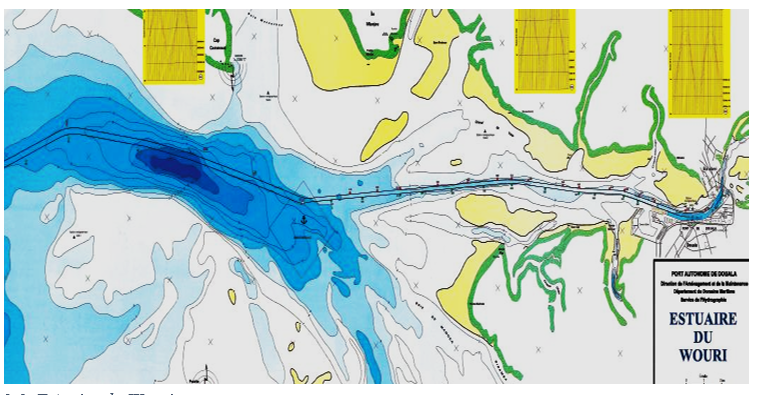
\includegraphics[width=1\textwidth,height=5in]{images/estuaireduWouri.png}
		%\includegraphics[width=0.8\textwidth]{images/estuaire du Wouri.png} % <-- remplace ce nom d'image%	
		\caption{Estuaire du Wouri\label{Fig 1}}
	\end{figure}
	
	
	
	
	\section*{V. Missions, objectifs et services du Port Autonome de Douala (PAD)}
	
	\section*{V.1 Missions}
	
	Le port de Douala est accessible par un long chenal de 50 km divisé en deux parties : 25 km à l’intérieur et 25 km à l’extérieur, balisé par des bouées lumineuses. Il assure la gestion, la promotion et le marketing du Port de Douala. À ce titre, il est chargé :
	
	\begin{enumerate}
		\item De la coordination générale des activités portuaires ;
		\item De l’assistance et de l’accueil des navires ;
		\item Des travaux d’équipements, d’extension, d’entretien du port ainsi que de la création et de l’aménagement des zones industrielles portuaires ;
		\item De la gestion, de la maintenance et du renouvellement des équipements portuaires qui lui sont affectés ;
		\item De la sécurité et de la police des opérations d’exploitation portuaire ;
		\item De la maîtrise d’ouvrage des travaux confiés aux entreprises spécialisées, y compris le dragage ;
		\item De la sûreté du chenal ;
		\item De la promotion de la place portuaire.
	\end{enumerate}
	
	\section*{V.2 Objectifs}
	
	\begin{enumerate}
		\item Le chenal intérieur, large de 150 m, est régulièrement dragué à la côte de -7 m. Des efforts sont en cours pour atteindre -8,5 m, permettant le passage de navires calant jusqu’à 11 m, grâce à l’amplitude des marées.
		
		\item Le PAD est engagé depuis plusieurs années dans un vaste processus de normalisation et de modernisation de ses infrastructures, visant à se hisser aux standards internationaux et à devenir un catalyseur de croissance économique nationale.
		
		\item « Le Port Autonome de Douala est engagé depuis quatre années dans un vaste processus de normalisation de toutes ses activités... », déclarait M. Cyrus NGO’O, Directeur Général du PAD, le 13 janvier 2021.
	\end{enumerate}
	
	\section*{V.3 Offre de services}
	
	\subsection*{1. Services aux navires}
	
	Le port fonctionne 24h/24 sous la supervision de la capitainerie. Les services fournis comprennent :
	\begin{enumerate}
		\item Aide à la navigation (chenal balisé et illuminé) ;
		\item Pilotage ;
		\item Remorquage et lamanage ;
		\item Avitaillement ;
		\item Réparation navale ;
		\item Chargement/déchargement ;
		\item Sécurité et surveillance.
	\end{enumerate}
	
	\subsection*{2. Services à la marchandise}
	
	Le PAD met à disposition :
	\begin{enumerate}
		\item 1000 ha de réserve foncière (600 ha exploités) ;
		\item 66 000 m² de magasins banalisés ;
		\item Plus de 10 millions de tonnes de capacité annuelle de traitement ;
		\item 15 millions de tonnes de capacité de stockage ;
		\item 80 000 m² de surface pour trafic conventionnel ;
		\item 10 km de quais ;
		\item Divers terminaux : conteneurs, bois, minéralier, fruitier, pêche, industrie ;
		\item 9 postes à quai pour trafic conventionnel ;
		\item 2 zones logistiques pour les hydrocarbures ;
		\item Zone industrielle portuaire (rive droite du Wouri) ;
		\item Zones d’entreposage longue durée ;
		\item 20 km de routes bitumées vers l’hinterland (Sud/Est/Ouest) ;
		\item 20 km de voies ferrées vers le Nord Cameroun, avec extension vers le Tchad et la RCA.
	\end{enumerate}
	
	\subsection*{3. Services divers}
	
	Le port abrite plus de 80\% des industries camerounaises, notamment :
	\begin{enumerate}
		\item \textbf{CIMENCAM} : transformation de clinker en ciment ;
		\item \textbf{DANGOTE} : idem ;
		\item \textbf{Les Grands Moulins} : transformation de blé en farine ;
		\item \textbf{COMETAL} : transformation du fer en carrosserie.
	\end{enumerate}
	
	\section*{V.4 Organisation de l’entreprise }
	
	Le Port Autonome de Douala est organisé de manière pyramidale, avec à sa tête :
	\begin{enumerate}
		\item Un Conseil d’administration ;
		\item Un Directeur Général ;
		\item Un Directeur Général Adjoint.
	\end{enumerate}
	
	Au centre de l’édifice, on retrouve plusieurs directions spécialisées. L'organigramme à la Figure \ref{Fig 2} illustre cette structure.
	
	\begin{figure}[h]
		\centering
		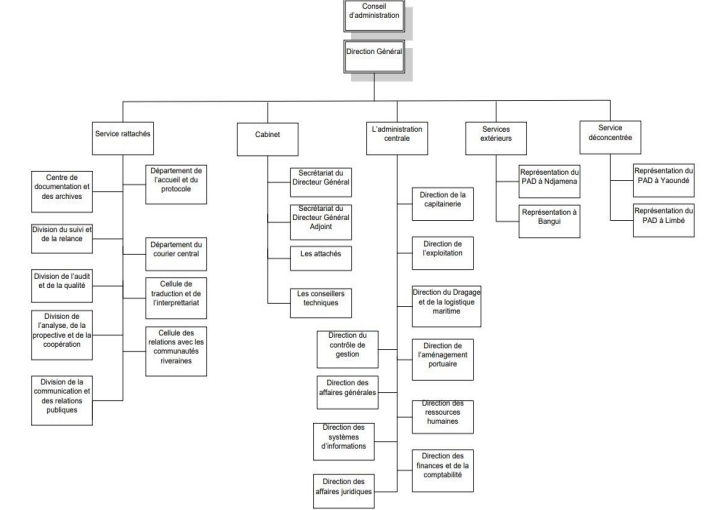
\includegraphics[width=0.99\textwidth]{images/orgramigrame_pad.png}
		\caption{Organigramme du PAD \label{Fig 2}}
	\end{figure}
	
	\section*{VI. Présentation de la Direction du Dragage et de la Logistique Maritime }
	
	La Direction du Dragage et de la Logistique Maritime   est placée sous l’autorité d’un Directeur, assisté éventuellement d’un Directeur Adjoint. Elle a pour mission de superviser toutes les activités relatives :
	
	\begin{enumerate}
		\item Aux travaux de dragage et maritimes ;
		\item À la logistique maritime ;
		\item À la sûreté et sécurité de navigation dans le chenal et les plans d’eau.
	\end{enumerate}
	
	Les principales responsabilités de la DDLM sont :
	
	\begin{enumerate}
		\item L’aménagement, la rénovation et l’entretien des infrastructures et superstructures maritimes, ainsi que leurs équipements ;
		\item Le dragage d’entretien et d’approfondissement ;
		\item La mise en place des aides à la navigation selon les normes AISM ;
		\item Le suivi des tirants d’eau et des plans de relevés de fonds ;
		\item La préparation des contrats de prestation (en lien avec les directions juridiques et financières) ;
		\item Le contrôle des travaux réalisés par des prestataires externes ;
		\item L’étude des phénomènes liés à l’environnement maritime ;
		\item La gestion de la maintenance du parc des engins nautiques ;
		\item Les relations avec la Marine Marchande et les sociétés de classification ;
		\item La logistique des engins nautiques.
	\end{enumerate}
%	
%

%========================================================================================================================= %

 \chapter*{LISTE DES ABRÉVIATIONS}
    \label{ch:listedesabbrévations}
    
    \addcontentsline{toc}{chapter}{LISTE DES ABRÉVIATIONS}
	\begin{flushleft}
	
\textbf{API} : \textbf{A}pplication \textbf{P}rogramming \textbf{I}nterface\\
\textbf{CAPC-AC} : \textbf{C}entre \textbf{D}'application pour les \textbf{P}révisions \textbf{C}limatiques en \textbf{A}frique \textbf{C}entrale\\
\textbf{CNN} : \textbf{C}onvolutional \textbf{N}eural \textbf{N}etwork\\
\textbf{CSV} : \textbf{c}omma \textbf{S}eparated \textbf{V}alues\\
\textbf{DMN} : \textbf{D}irection de la \textbf{M}étéorologie \textbf{N}ationale\\
\textbf{GEBCO} : \textbf{G}eneral \textbf{C}hart of the \textbf{O}ceans \textbf{M}odel\\
\textbf{GIEC} : \textbf{G}roupe \textbf{d'}\textbf{E}xperts \textbf{I}ntergouvernemental sur l'\textbf{É}volution du \textbf{C}limat\\
\textbf{GPS} : \textbf{G}lobal \textbf{P}ositioning \textbf{S}ystem\\
\textbf{GUI} : \textbf{G}raphical \textbf{U}ser \textbf{I}nterface\\
\textbf{IA} : \textbf{I}ntelligence \textbf{A}rtificielle\\
\textbf{LSTM} : \textbf{L}ong \textbf{S}hort \textbf{T}erm \textbf{M}emory\\
\textbf{MAE} : \textbf{M}ean \textbf{A}bsolute \textbf{E}rror\\
\textbf{MAPE} : \textbf{M}ean \textbf{A}bsolute \textbf{E}rror\\
\textbf{ML} : \textbf{M}achine \textbf{L}earning\\
\textbf{MongoDB} : \textbf{B}ase de \textbf{D}onnees \textbf{NoSQL} \textbf{O}rientée \textbf{D}ocument\\
\textbf{OMACC} : \textbf{O}bservatoire \textbf{N}ational sur les \textbf{C}hangements \textbf{C}limatiques\\
\textbf{OMI} : \textbf{O}rganisation \textbf{M}aritime \textbf{I}nternationale\\
\textbf{OMM} : \textbf{O}rganisation \textbf{M}étéorologique \textbf{M}ondiale\\
\textbf{ONR} : \textbf{O}bservation \textbf{N}ationale des \textbf{R}isques\\
\textbf{OpenWeather} : \textbf{P}lateforme de \textbf{D}onnées \textbf{M}étéorologiques en \textbf{L}igne\\
\textbf{PAD} : \textbf{P}ort \textbf{A}utonome de \textbf{D}ouala\\
\textbf{RCP} : \textbf{R}eprésentation \textbf{C}oncentration \textbf{P}athways\\
\textbf{RMSE} : \textbf{R}oot \textbf{M}ean \textbf{S}quared \textbf{E}rror\\
\textbf{SM2, SM3, SM4} : \textbf{S}tation \textbf{M}étéorologique \textbf{M}arégraphique 2,3 et 4 du \textbf{P}ort \textbf{A}utonome de \textbf{D}ouala\\
\textbf{Streamlit} : \textbf{F}ramework \textbf{P}ython pour \textbf{C}réer des \textbf{A}pplications \textbf{W}eb de \textbf{V}isualisation\\
\textbf{Tensorflow} : \textbf{B}ibliothèque \textbf{O}pen \textbf{S}ource de \textbf{M}achine \textbf{L}earning \textbf{D}éveloppée par \textbf{G}oogle\\
\textbf{UTC} : \textbf{C}oordinated \textbf{U}niversal \textbf{T}ime\\
\textbf{WRF} : \textbf{W}eather \textbf{R}esearch and \textbf{F}orecasting \textbf{M}odel\\
	\end{flushleft}

%======================================================================================================================= %

\chapter*{RÉSUMÉ} % Utilise * pour ne pas numéroter le chapitre dans le corps, mais l'ajoutera au TOC
\addcontentsline{toc}{chapter}{RÉSUMÉ} % Ajoute le titre au sommaire
	%\section{deee}
	\label{ch:abstract}
	%\addcontentsline{toc}{chapter}{Resumé}
	\phantomsection

	\quad Face à l’intensification des dérèglements climatiques et à la progression inexorable du niveau des mers, le Port autonome de Douala se retrouve à un tournant stratégique, exigeant des solutions prévisionnelles innovantes pour anticiper et maîtriser les risques environnementaux.
	Ce projet propose le développement d’un système intelligent de prévision météorologique conçu pour assurer la sécurité du trafic maritime tout en explorant de nouvelles opportunités économiques. Il s’appuie sur l’exploitation de données multisources, provenant à la fois de stations locales du port (SM2, SM3, SM4) et de plateformes externes telles qu’OpenWeatherMap, Windy et Copernicus.
	Un modèle d’apprentissage profond de type LSTM a été entraîné afin de prédire la température et les précipitations à court terme. Les données sont stockées dans une base MongoDB, accessible via une API Flask, garantissant flexibilité et rapidité d’accès. Par ailleurs, une interface web moderne, développée avec Streamlit et React, permet une visualisation dynamique et interactive des paramètres météorologiques, optimisant ainsi l’aide à la décision.
	La plateforme ainsi conçue vise une utilisation opérationnelle quotidienne et s’inscrit comme un outil stratégique pour les acteurs portuaires, maritimes et urbains, confrontés aux enjeux climatiques de plus en plus pressants.
	
	
	
	
	
	\textbf{Mots-clés }: \textbf{P}ort   \textbf{A}utonome de  \textbf{D}ouala ,\textbf{M}achine\textbf{L}earning , \textbf{I}ntelligence  \textbf {A}rtificielle, \textbf{L}ong \textbf{S}hort \textbf{T}erm \textbf{M}émory ,\textbf{A}pplication  \textbf{P}rogramming \textbf{I}nterface,\textbf{S}éries {T}emporelle, \textbf {P}révision    \textbf{M}étéorologique    


%======================================================================================================================= %	

\chapter*{ABSTRACT} % Utilise * pour ne pas numéroter le chapitre dans le corps, mais l'ajoutera au TOC
\addcontentsline{toc}{chapter}{ABSTRACT} % Ajoute le titre au sommaire	
	\label{ch:abstract}
	\label{ch:resume}
	
	\quad Faced with intensifying climate disruptions and the relentless rise in sea levels, the Autonomous Port of Douala stands at a strategic crossroads—calling for innovative forecasting solutions to anticipate and manage environmental risks.
	This project introduces the development of an intelligent weather forecasting system designed to ensure maritime traffic safety while exploring new economic opportunities. It relies on a fusion of data sources from local port stations (SM2, SM3, SM4) and external platforms such as OpenWeatherMap, Windy, and Copernicus.
	A deep learning model based on LSTM architecture has been trained to deliver short-term predictions for temperature and precipitation. Data is centralized in a MongoDB database and made accessible via a Flask API, ensuring flexibility and fast retrieval. Additionally, a modern web interface, developed using Streamlit and React, offers dynamic and interactive visualization of meteorological parameters to enhance decision-making.
	The platform is built for daily operational use, positioning itself as a strategic tool for stakeholders in port, maritime, and urban sectors confronting increasingly pressing climate challenges.
	\\
	
	
		\textbf{Keywords}: \textbf{D}ouala \textbf{A}utonomous \textbf{P}ort, \textbf{M}achine \textbf{L}earning, \textbf{A}rtificial \textbf{I}ntelligence, \textbf{L}ong \textbf{S}hort \textbf{T}erm \textbf{M}emory, \textbf{A}pplication \textbf{P}rogramming \textbf{I}nterface, \textbf{T}ime \textbf{S}eries, \textbf{W}eather \textbf{F}orecasting
	
	\clearpage \phantomsection

 \newpage\pagenumbering{arabic}

%======================================================================================================================== %
\chapter*{INTRODUCTION GÉNÉRALE }\addcontentsline{toc}{chapter}{INTRODUCTION}
%\chapter{Introduction Générale}
\label{chap:intro}

	Le changement climatique, l'urbanisation rapide et la pression croissante sur les zones côtières rendent la prévision météorologique plus que jamais indispensable, notamment dans des villes comme Douala. En tant que principal port maritime du Cameroun et plaque tournante de l'économie nationale, Douala est particulièrement exposée aux phénomènes climatiques extrêmes (précipitations intenses, houles, montée du niveau des eaux), susceptibles d'affecter la sécurité portuaire, les activités de pêche, le transport maritime ainsi que les infrastructures côtières. Or, les systèmes de prévision actuellement disponibles sont souvent globaux, peu localisés ou limités dans leur accessibilité en temps réel. Cette problématique met en lumière la nécessité de concevoir une solution locale, automatisée, intégrant à la fois des données collectées en temps réel sur le terrain et des algorithmes d'intelligence artificielle adaptés à la nature séquentielle des phénomènes météorologiques.
	\quad Le changement climatique, l’urbanisation rapide et la pression croissante sur les zones côtières rendent la prévision météorologique  plus que jamais indispensable, notamment dans des villes comme Douala. En tant que principal port maritime du Cameroun et plaque tournante économique, Douala est particulièrement exposée aux phénomènes climatiques extrêmes (précipitations intenses, houles, montée des eaux) qui peuvent affecter la sécurité portuaire, les activités de pêche, le transport maritime, ainsi que les infrastructures côtières.Or, les systèmes de prévision disponibles sont souvent globaux, peu localisés, ou limités dans leur accessibilité en temps réel. Cette problématique soulève la nécessité de concevoir une solution locale, automatisée, intégrant à la fois des données collectées en temps réel sur le terrain et des algorithmes d’intelligence artificielle adaptés à la nature séquentielle des phénomènes météorologiques.

\section{Contexte général et Objectifs}
	
\subsection{Contexte général}
%gpt
	\quad
	Dans un contexte mondial marqué par l’augmentation des événements météorologiques extrêmes (pluies intenses, houles, submersions, etc.), les régions côtières comme celle de Douala deviennent particulièrement vulnérables aux aléas climatiques. Ces phénomènes affectent non seulement la sécurité des infrastructures portuaires, mais aussi les activités économiques liées au commerce maritime, à la pêche ou encore à la gestion urbaine. Face à ces enjeux, les technologies d’intelligence artificielle, et en particulier les modèles de \emph{deep learning} comme le LSTM (\textit{Long Short-Term Memory}), offrent de nouvelles perspectives pour analyser et prédire les séries temporelles météorologiques avec une précision accrue. En parallèle, la vulgarisation des outils de visualisation web comme \texttt{Streamlit} et \texttt{React} permet de rendre ces données accessibles et compréhensibles pour les utilisateurs finaux.
	
	\medskip
	
	Notre travail s’inscrit ainsi dans une démarche d’aide à la décision en temps réel, en combinant :
	\begin{enumerate}
		\item la collecte automatisée de données météo à partir d'OpenWeatherMap ;
		\item l’entraînement d’un modèle prédictif LSTM multivarié pour la température et les précipitations ;
		\item le développement d’une interface web interactive de visualisation et de diffusion en temps réel des prévisions ;
		\item l’intégration d’outils de prévision tiers (Windy, Copernicus) pour enrichir l’analyse ;
		\item et la conception d’une application web interactive pour la visualisation, l’analyse et la diffusion quotidienne des prévisions.
	\end{enumerate}
	
 
	
\subsection{Objectif général}
	\quad 	Ce travail consiste à développer une solution complète de prévision  de l'état de l'atmosphère au   port Autonome de Douala, en combinant des données locales, un modèle prédictif basé sur les réseaux LSTM et une interface web interactive\\

	
\subsection{Objectifs Spécifiques}
	
\begin{enumerate}
	\item Structurer les données météorologiques et marégraphiques issues des stations SM2, SM3 et SM4 du Port autonome de Douala, ainsi que celles provenant de sources ouvertes comme OpenWeatherMap;
	
	\item Mettre en œuvre un processus de prétraitement des données (nettoyage, normalisation, séquençage), adapté aux modèles de séries temporelles multivariées;
	
	\item Concevoir, entraîner et valider un modèle d’apprentissage profond de type LSTM pour la prédiction à court terme de la température et des précipitations;
	
	\item Développer une plateforme web permettant la visualisation des données, l’affichage des prévisions et l’accès à des outils d’aide à la décision.
\end{enumerate}
	\quad
	
	La prévision des conditions météorologiques et maréographiques est un enjeu crucial pour les activités portuaires, notamment dans les zones côtières à forte dynamique comme le Port Autonome de Douala. L’évolution des techniques d’intelligence artificielle et l’accessibilité croissante des données ouvertes (open data) offrent aujourd’hui de nouvelles perspectives pour améliorer la précision des prévisions dans ces environnements complexes.
	
	Ce mémoire s’inscrit dans cette dynamique en proposant une démarche innovante de modélisation prédictive des variables météorologiques  à l’aide d’algorithmes de machine learning, avec une application concrète au Port Autonome de Douala.
	
	
\quad Le présent travail est structuré comme suit: Le Chapitre \ref{chap:Etat_Art} est consacré à l’état de l’art des modèles de prévision météorologique , avec un accent particulier sur les approches par apprentissage automatique; Le Chapitre \ref{chap:Methode} décrit les données utilisées, leur provenance, ainsi que les étapes de nettoyage et de prétraitement nécessaires à leur exploitation; Le Chapitre \ref{ch:résultatsetdiscussion} expose la méthodologie de modélisation adoptée, incluant les choix algorithmiques (LSTM, BiLSTM, ARIMA) et les métriques d’évaluation et  présente l’implémentation d’une plateforme web interactive pour la visualisation des données et des prévisions en temps réel. Enfin, une conclusion générale vient récapituler les principaux résultats obtenus, leurs limites, et proposer des perspectives d’amélioration.
	
	
	

    
%====================================================================================================================%
\chapter{ÉTAT DE L'ART }
\label{chap:Etat_Art}	

		\section*{}
	

	 \quad Dans un contexte mondial marqué par l'accélération des dérèglements climatiques, la maîtrise des paramètres météorologiques et marégraphiques constitue un enjeu stratégique pour les zones côtières à forte densité d'activités économiques, notamment les ports \cite{Nicholls2008}. Le Port autonome de Douala est particulièrement vulnérable aux variations du niveau de la mer, aux précipitations extrêmes et aux tempêtes côtières \cite{Ngatcha2021}. Les avancées récentes en matière de technologies d'observation, combinées à la modélisation mathématique et à l'intelligence artificielle, offrent de nouvelles perspectives pour anticiper et gérer ces phénomènes \cite{Bremnes2020}. Ainsi, l'introduction du \textit{machine learning} dans le traitement des séries temporelles environnementales ouvre la voie à des prévisions plus fines, plus réactives et mieux contextualisées localement \cite{Shamshirband2020}.
	
	\section{Le contexte portuaire et ses enjeux environnementaux}
	
	\subsection{ Contexte portuaire }
	
	\quad Le Port Autonome de Douala, joue un rôle stratégique dans l'économie nationale et sous-régionale. Situé dans l'estuaire du Wouri, il assure environ 95 \% du trafic maritime national et constitue un axe de transit majeur pour les pays enclavés tels que le Tchad et la République Centrafricaine \cite{PAD2023}. Cette localisation lui confère une importance logistique mais aussi une vulnérabilité accrue aux variations naturelles telles que les marées, les crues et l'érosion côtière  \cite{Bruckmann2019} .  \\

	\quad  
	Le PAD est également un centre d'activités complexes (commerce, pêche, hydrocarbures, douanes, etc.), ce qui nécessite une planification efficace des opérations portuaires. Ces activités sont fortement conditionnées par les facteurs météorologiques et marins, comme la visibilité, le vent, les vagues, ou encore les niveaux d'eau \cite{OMM2023} .\\
	

	
	\subsection{Enjeux environnementaux }
	
	
	\quad Le littoral camerounais est exposé à de nombreux aléas naturels, tels que l’élévation du niveau de la mer, les tempêtes tropicales et les inondations. Ces phénomènes sont exacerbés par les effets du changement climatique, notamment dans la zone côtière de Douala, où les précipitations abondantes, combinées à un réseau de drainage urbain insuffisant, aggravent considérablement les risques d’inondation \cite{Bruckmann2019}.
	
	\quad Par ailleurs, la pollution marine et les activités anthropiques (dragage, rejet d’eaux usées, déforestation des mangroves) affectent la biodiversité et perturbent les équilibres naturels du port \cite{PNUE2021}.
	
	
	\section{Données météorologiques et marégraphiques }
	\subsection{  Types de données météorologiques }
	
	\quad Les données météorologiques utilisées dans les systèmes de prévision portuaire incluent principalement : la température de l’air, la pression atmosphérique, l’humidité relative, la direction et la vitesse du vent, les précipitations, la visibilité, et parfois la couverture nuageuse \cite{OMM2018}. Ces variables sont mesurées à l’aide de capteurs installés sur des stations météorologiques automatisées, souvent couplées à des instruments GPS pour la géolocalisation \cite{Pena2020}. Ces informations sont généralement collectées à intervalles réguliers (toutes les 10 à 60 minutes), afin de permettre des analyses de séries temporelles et la détection éventuelle d’anomalies. Elles sont cruciales pour les manœuvres portuaires, la sécurité des navires à quai ou en approche, ainsi que pour la planification des escales \cite{Pena2020}.
	
	
	
	
	\subsection{Types de données marégraphiques}
	
	\quad Les données marégraphiques désignent les mesures du niveau de la mer en un point donné, généralement obtenues grâce à des capteurs marégraphiques — à radar ou à pression — installés sur les quais ou les bouées \cite{COIUNESCO2016}. Les variables associées comprennent le niveau moyen de la mer, les hauteurs de marée, la période des vagues, et parfois les vitesses des courants marins \cite{Pugh2014}.
	
	\quad Dans les ports tropicaux comme Douala, ces données sont sensibles aux effets de la marée semi-diurne, aux variations saisonnières induites par les précipitations, ainsi qu’aux remontées d’eau liées à l’embouchure du fleuve Wouri \cite{Ngatcha2021}.
	
	
	\quad Ils se divisent principalement en deux catégories : les données de hauteur de la surface marine et les données de mesures associées. Les premières peuvent être instantanées ou moyennes sur une période donnée, et sont enregistrées par des marégraphes de surface ou immergés. Les secondes incluent la pression, la température et la conductivité de l’eau, ainsi que la pression atmosphérique.
	


	\subsection{Importance des données météorologiques et  marégraphiques}
	
\quad L’exploitation des données météorologiques et marégraphiques permet d’anticiper les conditions critiques pour les opérations portuaires, telles que les vents violents pouvant gêner l’accostage ou le déchargement des navires, ou encore les épisodes de fortes pluies susceptibles de provoquer des interruptions logistiques \cite{Tang2021}. À long terme, ces données permettent également de modéliser des tendances climatiques locales, utiles pour la planification des infrastructures portuaires \cite{Oueslati2019}.

\quad Dans le cas du PAD, la connaissance en temps réel de la vitesse et de la direction du vent, par exemple, constitue un paramètre essentiel pour le pilotage et la sécurité maritime dans l’estuaire du Wouri \cite{PAD2023}. L’exploration de nouvelles voies en météorologie maritime nous permet de nous projeter dans le futur et d’approfondir notre compréhension de l’état de l’atmosphère.

\begin{enumerate}
	\item \textbf{Évolution du climat mondial à long terme :}
	
	\quad Selon la Figure \ref{Fig 1.1} ,Les courbes pleines représentent les anomalies (écarts) de la température moyenne mondiale de l’air, tandis que les courbes pointillées illustrent l’élévation du niveau de la mer due à la dilatation thermique des océans (appelée élévation thermostérique). Les zones ombrées mettent en évidence les horizons temporels d’intérêt et leurs années de référence nominales. L’image du bas montre les anomalies spatiales par rapport à la moyenne 2000–2019 pour les climats de 2100, 2200 et 2500 selon les trois scénarios RCP \cite{Lyon2021}.
	
	\quad Le manque de données marégraphiques et météorologiques fiables peut ne pas être la cause directe d’un chavirage, mais il constitue un facteur aggravant dans plusieurs incidents maritimes. Voici quelques exemples illustrant  :\\
	
	\quad \textbf{- Le chavirage du trimaran \emph{Solidaires en Peloton – ARSEP} (2024)}
	Ce trimaran de la classe \emph{Ocean Fifty} a chaviré au sud de l’Espagne lors d’un convoyage de retour voir Figure\ref{Fig 1.2} . Le skipper Thibaut Vauchel-Camus a expliqué que le bateau a fait un « soleil » en pleine nuit, probablement à cause d’un déséquilibre soudain ou d’une rafale mal anticipée.
	%\vspace{0.5em}
	Cependant,les causes sont  :\textbf{Conditions météorologiques extrêmes} : vents forts, bourrasques ou orages; \textbf{Erreur de navigation ou de stratégie} : mauvaise évaluation des trajectoires ou des phénomènes météo;\textbf{Problèmes techniques ou mécaniques} : défaillances d’équipements ou problèmes structurels ; \textbf{Mauvaise gestion du vent ou des vagues} : surtout lors de manœuvres à haute vitesse \cite{Bianchi2017}.\\
	\quad \textbf{- Le cas du Cougar Ace (2006)   }
	Representé sur la Figure \ref{fig1.3} ,ce navire transportant des véhicules a chaviré au large de l’Alaska lors d’un transfert de ballast. Bien que l’incident soit principalement lié à une mauvaise gestion de la stabilité, une meilleure connaissance des conditions locales, y compris les variations du niveau de la mer, aurait pu contribuer à éviter l’accident\cite{USCG2006}.
\end{enumerate}

\begin{figure}[H]
	\begin{center}
		 \begin{minipage}{\textwidth}
		    \begin{center}
		    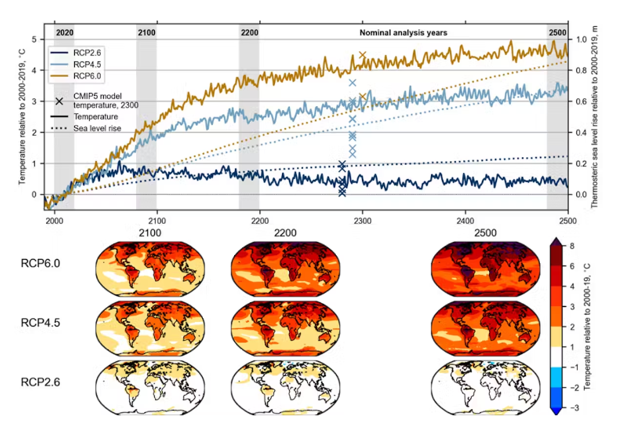
\includegraphics[width=1\textwidth,height=4.6in]{images/Anomilie_de_T.png}
		    \end{center}
		    \end{minipage}
		
		\caption{\emph{ Anomalies de la température moyenne mondiale de l’air(lignes pleines) et de l'élévation thermostérique du niveau de la mer (lignes pointillées) par rapport à la moyenne de 2000-19 pour les scénarios RCP6.0, RCP4.5 et RCP2.6.\cite{Bianchi2017}\label{Fig 1.1} }} 
	\end{center}
\end{figure}
\quad\textbf{-Le naufrage du MV Derbyshire (1980) }:Ce vraquier britannique a coulé en mer de Chine méridionale avec 44 personnes à bord. Bien que les causes aient été attribuées à des vagues extrêmes, les enquêtes ont révélé un manque de données précises sur les pressions sous-marines et les hauteurs de vagues, ce qui a limité la compréhension des mécanismes de rupture de la coque. Cet événement a conduit à une amélioration des systèmes de mesure océanographique et à la reconnaissance de l’importance des données marégraphiques dans la conception navale\cite{Gaillarde2001},nous avons ces épaves a la Figure \ref{fig1.4}.

\textbf{-Ports d’Afrique de l’Ouest }:Des rapports de l’UNESCO et de l’OMI ont souligné que le manque de stations marégraphiques fiables dans des ports comme ceux du Golfe de Guinée augmente les risques pour les navires, notamment lors des manœuvres en période de marée mal anticipée. L’absence de données en temps réel peut compromettre la sécurité des opérations portuaires.\\
\quad Parlant des Normes de stabilité et conception navale,des articles spécialisés, comme celui de Chasse Marée, rappellent que la stabilité d’un navire dépend aussi de la connaissance précise des conditions maritimes, y compris les marées. L’application de normes comme l’ISO 12217 repose sur des données fiables pour évaluer la résistance au chavirement.\\

  
\begin{figure}[H]
	\begin{center}
	           \begin{minipage}{\textwidth}
			    \begin{center}
			    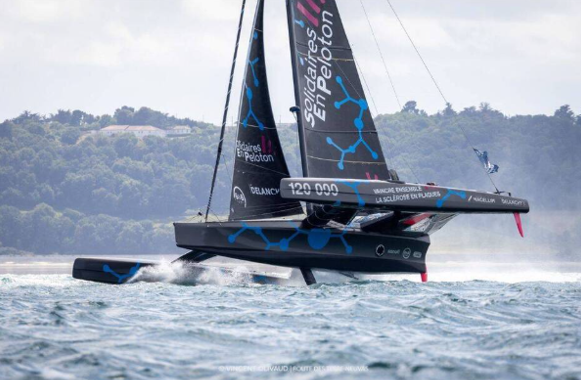
\includegraphics[width=1\textwidth,height=4.6in]{images/trimaran.png}
			    \end{center}
			    \end{minipage}
			\caption{\emph{Le trimaran Solidaires en Peloton – ARSEP a chaviré fin 2024, apparemment au large de l'Espagne\cite{Bianchi2017}\label{Fig 1.2} }} 
	\end{center}
\end{figure}
%%%%%%%%%%%%%%%%%%%%%%%%%%%%%%%%%%%%%%%%%%%%
\begin{table}[htbp]
	\centering
	\caption{Accidents de navires au Port Autonome de Douala (2017–2021)}
	\begin{tabular}{|c|c|c|p{7cm}|}
		\hline
		\textbf{Année} & \textbf{Nombre d'accidents} & \textbf{Évolution annuelle} & \textbf{Observations possibles} \\
		\hline
		2017 & 12 & --- & Année la plus accidentogène \\
		\hline
		2018 & 6 & ↓ 50\,\% & Forte réduction \\
		\hline
		2019 & 5 & ↓ 16{,}7\,\% & Stabilisation progressive \\
		\hline
		2020 & 4 & ↓ 20\,\% & Maintien de la baisse \\
		\hline
		2021 & 4 & = & Niveau stable, mais vigilance toujours requise \\
		\hline
	\end{tabular}
	\label{tab:douala_accidents}
\end{table}

\quad 
Nous avons des ports qui ont augmenté leurs chiffres d'affaire en intégrant la météo dans leurs espace portuaire,nous pouvons parler de :\\
\quad
\textbf{- HAROPA PORT (France) }:Le groupement HAROPA (Le Havre, Rouen, Paris) a vu son chiffre d’affaires grimper à  437 millions d’euros en 2024 , en hausse de 3,6 \%. Cette croissance est liée à une meilleure gestion logistique, notamment grâce à des outils numériques intégrant des données météorologiques et maritimes pour optimiser les escales, les transbordements et les flux multimodaux(HAROPA PORT. (2025)\cite{GPFMA2024}.

\quad
\textbf{- Port d’Itajaí (Brésil)}:En 2017, ce port a dû fermer pendant près d’un mois à cause de fortes précipitations. Depuis, il a investi dans des systèmes de prévision météorologique et hydrologique pour anticiper les événements extrêmes. Ces mesures ont permis de  réduire les interruptions d’activité , ce qui a un impact direct sur la performance économique\cite{Murara2018}.

\quad
\textbf{-Port de Rotterdam (Pays-Bas)}:Bien qu’aucun chiffre précis ne soit cité ici, Rotterdam est un pionnier dans l’utilisation de  jumeaux numériques  intégrant des données météo, marégraphiques et logistiques. Cela permet d’optimiser les fenêtres d’accostage et de réduire les temps d’attente, ce qui améliore la productivité globale\cite{Rotterdam2018}.
\quad Les données marégraphiques sont tout aussi importantes, car elles conditionnent directement l’accessibilité des quais et des chenaux d’accès portuaires. Une faible marée peut interdire à certains navires de manœuvrer, tandis qu’une surcote marine due à une tempête peut submerger des installations côtières et conduire à des accidents Voir les Tableaux (\ref{tab:douala_accidents};\ref{tab:comparaison_ports} et \ref{tab:levers-perf-percent} )\cite{Martins2019}.
	\begin{table}[h!]
\caption{Évaluation comparative des ports selon  trois leviers de performance}
	\centering
	
	\begin{tabular}{|l|c|c|c|}
		
		\hline
		\textbf{Port}     & \textbf{Météorologie} & \textbf{Réduction pertes} & \textbf{Logistique} \\
		\hline
		Douala            & 3/5                   & 3/5                        & 2.5/5               \\
		\hline
		Rotterdam (PB)        & 5/5                   & 4.75/5                     & 5/5                 \\
		\hline
		Itajaí  (Brésil)          & 4.5/5                 & 4.75/5                     & 4.5/5               \\
		\hline
		HAROPA  (France )         & 4.75/5                & 4.5/5                      & 4.75/5              \\
		\hline
	\end{tabular}

	\label{tab:comparaison_ports}
\end{table}

\begin{figure}[H]
	\begin{center}
	                  \begin{minipage}{\textwidth}
	     			  \begin{center}
	     			  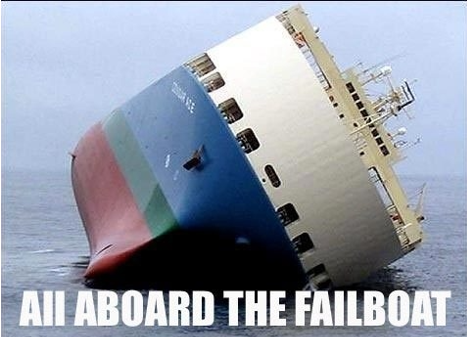
\includegraphics[width=1\textwidth,height=4in]{images/MC_cougar_ace.png}
	     			    \end{center}
	     			    \end{minipage}
		\caption{\emph{Le MV Cougar Ace, un roulier battant pavillon singapourien, a connu un incident notable en 2006 \cite{USCG2006}.\label{fig1.3} }} 
	\end{center}
\end{figure}

\begin{table}[h!]
\caption{Évaluation comparative des ports selon trois leviers exprimée en pourcentages}
	\centering
	\begin{tabular}{|l|c|c|c|}
		\hline
		\textbf{Port} & \textbf{Météorologie (\%)} & \textbf{Réduction pertes (\%)} & \textbf{Logistique (\%)} \\
		\hline
		Douala(2023)    & 60\%  & 60\%  & 50\%  \\
		\hline
		Rotterdam & 100\% & 95\%  & 100\% \\
		\hline
		Itajaí    & 90\%  & 95\%  & 90\%  \\
		\hline
		HAROPA    & 95\%  & 90\%  & 95\%  \\
		\hline
	\end{tabular}
\label{tab:levers-perf-percent}
\end{table}
\begin{figure}[H]
	\begin{center}
		\begin{minipage}{\textwidth}
			\begin{center}
				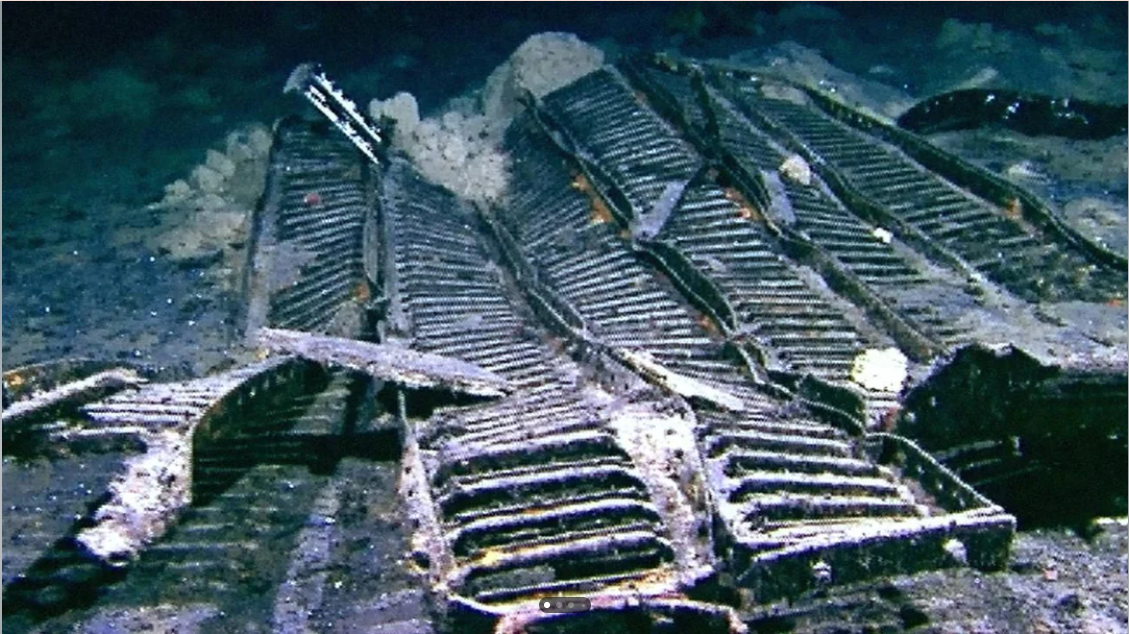
\includegraphics[width=0.9\textwidth,height=3in]{images/Epave_derbyshire.png}
			\end{center}
		\end{minipage}
		\caption{Epave du  Derbyshire,il a fait route dans le typhon Orchid, à environ 230 miles (370 km) d'Okinawa, et a été submergé par la tempête tropicale, tuant tous à bord \cite{Gaillarde2001}. \label{fig1.4}} 
	\end{center}
\end{figure}


	
	\section{Intelligence Artificielle et Machine Learning}
	\subsection{  Définitions }
	\quad L’Intelligence Artificielle est un domaine de l’informatique qui vise à créer des systèmes capables d’accomplir des tâches nécessitant normalement l’intelligence humaine, telles que la reconnaissance vocale, la prise de décision, l’apprentissage ou la compréhension du langage \cite{Russell2020}.Elle englobe des sous-domaines tels que la robotique, le traitement automatique des langues, la vision par ordinateur et l’apprentissage automatique (machine learning).Le Machine Learning  est une branche de l’IA qui consiste à entraîner des algorithmes à partir de données, afin qu’ils puissent faire des prédictions ou prendre des décisions sans avoir été explicitement programmés pour cela voir la figure \ref{Fig 1.5 } \cite{Mitchell1997}. Il s’appuie sur des techniques statistiques et algorithmiques pour extraire des relations cachées dans les données  . \\
	\begin{figure}[H]
		\begin{center}
	    	    \begin{minipage}{\textwidth}
	    	     \begin{center}
	    	      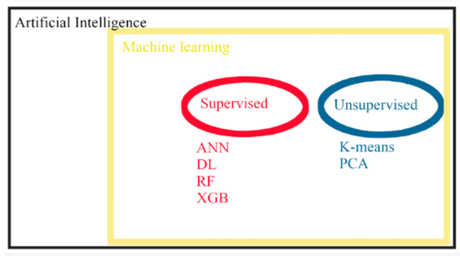
\includegraphics[width=0.9\textwidth,height=2.5in]{images/Inteligence_Artificielle.png}
	    	      \end{center}
	    	     \end{minipage}
			\caption{\emph{Représentation global de l'IA \cite{Mitchell1997} \label{Fig 1.5 }}}
		\end{center}
	\end{figure}%
	\subsection{Évolution de l’intelligence artificielle}
		\begin{figure}[H]
		\begin{center}
	    	    \begin{minipage}{\textwidth}
	    	     \begin{center}
	    	      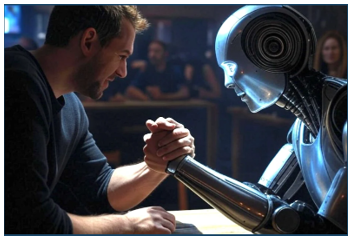
\includegraphics[width=1\textwidth,height=4.6in]{images/IA_vas_nous_remplacer.png}
	    	      
	    	      \end{center}
	    	     \end{minipage}
			
			\caption{Comparaison de l'IA et l'Homme\cite{Goodfellow2016}\label{Fig 1.6}}
		\end{center}
	\end{figure}%
 \quad Le développement de l’IA a connu plusieurs phases, marquées par des avancées techniques et des périodes de stagnation appelées "AI winters". Les débuts remontent aux années 1950 avec des pionniers comme Alan Turing et John McCarthy.Cependant, c’est dans les années 2010 que l’IA a connu une accélération significative, grâce à l’explosion des volumes de données (big data), à la puissance de calcul accrue  et à la généralisation des réseaux de neurones profonds (deep learning) \cite{Goodfellow2016}.
	Aujourd’hui, l’IA est appliquée dans des domaines aussi variés que la santé, les transports, la finance ou encore la prévision environnementale, notamment pour l’analyse de séries temporelles climatiques  \cite{LeCun2015} .
	\quad L’intelligence artificielle ne vise pas à remplacer l’humain, mais plutôt à automatiser certaines tâches, souvent répétitives, dangereuses ou très complexes. Par exemple, dans des domaines comme la médecine, l’aviation ou la logistique portuaire, l’IA peut analyser des volumes massifs de données pour aider à la prise de décision, sans pour autant se substituer à l’expertise humaine voir Figures \ref{Fig 1.7}.

	 		\begin{figure}[H]
		\begin{center}
                \begin{minipage}{\textwidth}
	    	     \begin{center}
	    	      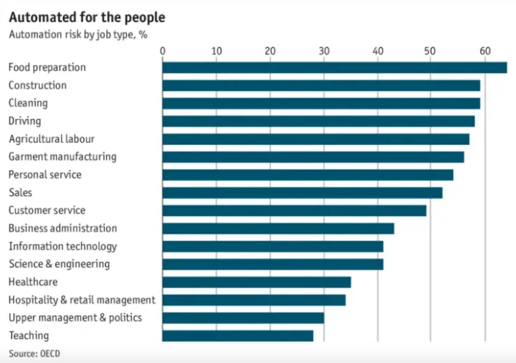
\includegraphics[width=1\textwidth,height=4.6in]{images/Impact_de_IA .png}
	    	      \end{center}
	    	     \end{minipage}
			
			\caption{Impact de l’IA sur l’emploi  \cite{LeCun2015}\label{Fig 1.7}}
		\end{center}
	\end{figure}%
	

	\subsection{Le machine learning appliqué aux séries temporelles environnementales}
	
	\quad Les séries temporelles sont des ensembles de données chronologiques dans lesquelles les observations sont indexées dans le temps. En météorologie et en marégraphie, ces séries sont essentielles pour détecter des tendances, anomalies ou régularités \cite{Hyndman2018}.Le machine learning permet d’exploiter ces séries pour la modélisation prédictive. Des algorithmes comme les régressions linéaires, les forêts aléatoires (random forests), ou les réseaux de neurones récurrents  sont capables de prédire les valeurs futures à partir d’un historique de données\cite{Zhang2020} .
	Ces modèles apprennent automatiquement les comportements complexes, parfois non linéaires, qui régissent les phénomènes naturels tels que les marées, les vents ou les précipitations.
	
	
	\subsection{Modèle CNN 1D}
	
	Le \textbf{réseau de neurones convolutif unidimensionnel (CNN 1D)} est un modèle d’intelligence artificielle particulièrement adapté à l'analyse des \textit{données temporelles} ou séquentielles, telles que celles issues des mesures météorologiques ou marégraphiques. Contrairement aux CNN 2D utilisés pour le traitement d’images, le CNN 1D opère sur des vecteurs de séries temporelles en appliquant des \textit{filtres convolutifs} qui permettent de détecter automatiquement des \textit{motifs locaux} (pics, variations brusques, tendances cycliques). Ce modèle est reconnu pour sa \textit{rapidité d’apprentissage}, sa \textit{robustesse face au bruit}, ainsi que sa capacité à \textit{extraire efficacement les caractéristiques pertinentes}, même à partir de données partiellement bruitées ou incomplètes \cite{Kiranyaz2015}.Dans le cadre de la \textit{modélisation prédictive des conditions environnementales}, plusieurs études ont démontré l'efficacité des CNN 1D, notamment pour la \textit{prévision climatique, marégraphique ou d’événements extrêmes}. Par exemple,\cite{Yu2022} montrent que les CNN 1D surpassent les approches classiques de prévision météorologique à court terme, en capturant efficacement les tendances saisonnières et les fluctuations rapides. Ce modèle s’avère donc particulièrement pertinent dans un contexte comme celui du Port Autonome de Douala, où une \textit{prévision précise des conditions météo-marégraphique} est essentielle pour assurer la \textbf{sécurité maritime} et optimiser les opérations portuaires. 
	

		\subsection{Modèle BiLSTM}
		
		Le modèle \textbf{BiLSTM} (\textit{Bidirectional Long Short-Term Memory}) est une extension du modèle LSTM classique, conçue pour traiter efficacement les \textit{données temporelles dans les deux directions du temps} : passée et future. Alors que le LSTM classique n’exploite que les dépendances dans une seule direction temporelle (typiquement du passé vers le futur), le BiLSTM combine deux réseaux LSTM parallèles, dont l’un traite la séquence dans le sens direct et l’autre dans le sens inverse. Cette approche permet de capturer des \textit{relations temporelles plus riches et plus complètes}, ce qui est particulièrement utile dans les systèmes de prévision environnementale où les phénomènes peuvent dépendre d’un \textit{contexte temporel plus large} \cite{Graves2005}.Dans le domaine de la \textit{prédiction météorologique et hydrologique}, le BiLSTM a montré des performances supérieures aux modèles unidirectionnels, notamment pour la prévision de séries temporelles complexes telles que les précipitations, la température ou le niveau de marée. Par exemple, \cite{Zhang2021} ont démontré que les BiLSTM surpassent les LSTM simples dans la modélisation de séries climatiques multivariées, grâce à leur capacité à intégrer les signaux passés et futurs dans chaque prédiction. Ce type de modèle est donc particulièrement pertinent dans le cadre d’un système intelligent de \textbf{prévision météo-marégraphique pour le Port Autonome de Douala}.
		
		
	
		\subsection{ Modèle LSTM}
                         
	\quad Les Long Short-Term Memory sont une architecture particulière des RNN conçue pour surmonter le problème du "gradient qui disparaît" \cite{Hochreiter1997}.Ils possèdent des mécanismes appelés "portes" (qui sont comme des filtres automatiques ) qui régulent le flux d’information, permettant au réseau de retenir ou d’oublier certaines informations sur de longues périodes.Les LSTM sont particulièrement efficaces dans le domaine des prévisions environnementales, car ils sont capables de mémoriser les cycles temporels comme les cycles de marée ou les tendances saisonnières , tout en réagissant à des changements brusques comme les événements extrêmes météorologiques \cite{Bianchi2017}.
	Dans le contexte du Port Autonome de Douala, l’utilisation d’un LSTM permettrait de modéliser avec précision les conditions météorologiques et marégraphiques en prenant en compte la variabilité temporelle propre à la zone \cite{Wang2021}.
	pour illuster ces modèles  voir Figure \ref{Fig 1.8} .
		\begin{figure}[H]
		\begin{center}
			\begin{minipage}{\textwidth}
				\begin{center}
					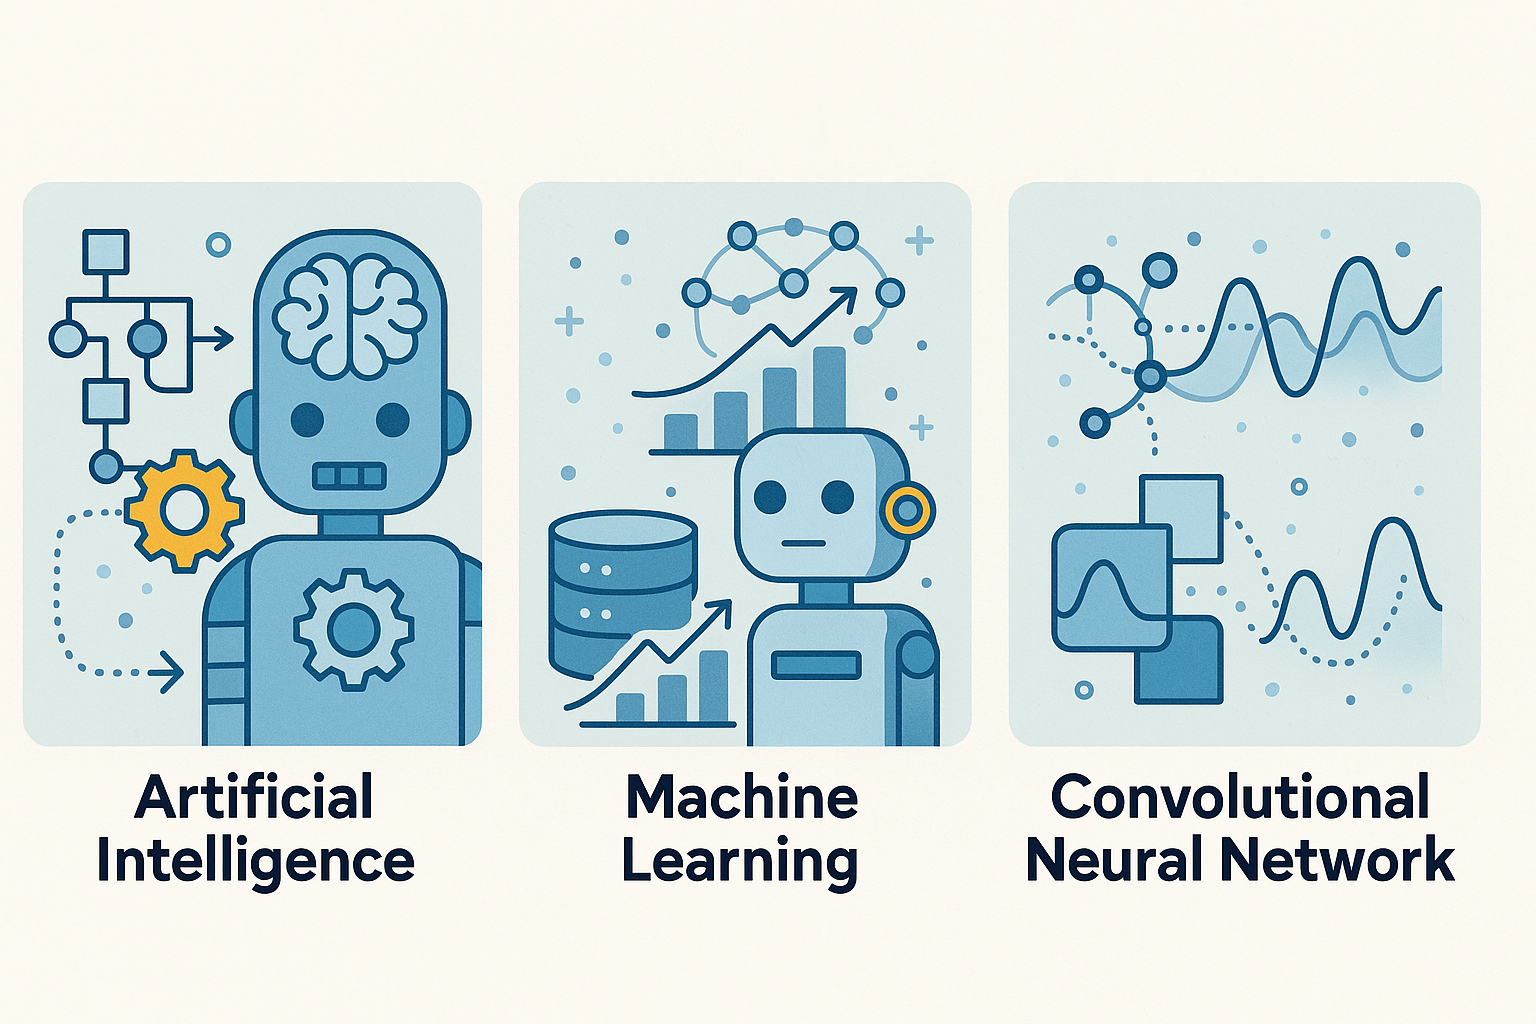
\includegraphics[width=1\textwidth,height=4.6in]{images/an abstract represen.png}
				\end{center}
			\end{minipage}
			
			\caption{CNN \& ML \& IA \cite{Abraham2019}\label{Fig 1.8}}
		\end{center}
	\end{figure}%
	
	\begin{minipage}{\textwidth}
	
	\end{minipage}
	
\section{Prévision marégraphique et météorologique}

	\subsection{Prévision des niveaux d’eau}
	
	\quad La prévision des marées repose historiquement sur l’analyse harmonique, une méthode qui décompose les niveaux marins en une somme d’ondes sinusoïdales liées à l’attraction gravitationnelle de la Lune et du Soleil \cite{Pugh2014}.
	Toutefois, cette approche atteint ses limites dans les zones portuaires complexes où les interactions entre les facteurs astronomiques et météorologiques sont non linéaires. D’où l’intérêt de méthodes plus modernes fondées sur l’apprentissage automatique\cite{Fernandes2020}.Les réseaux de neurones, notamment les modèles LSTM, permettent aujourd’hui de prédire le niveau de la mer avec une grande précision en intégrant aussi bien les composantes astronomiques que les influences atmosphériques telles que la pression ou le vent\cite{Wang2021} 
	\subsection{Prévision des marées}
	\quad La prévision des niveaux d’eau dans les estuaires et les zones côtières comme le Port de Douala est un enjeu crucial pour la sécurité maritime et la gestion des infrastructures\cite{Ngatcha2021} .Les facteurs qui influencent le niveau de l’eau sont multiples : marée, débit fluvial, pression atmosphérique, vent, et houle\cite{Zhou2022}
	Des modèles hybrides combinant données in-situ et modèles statistiques ou réseaux neuronaux profonds sont de plus en plus utilisés dans les ports tropicaux. Ils permettent d’anticiper les périodes de submersion ou d’étiage et d’ajuster les opérations portuaires en conséquence \cite{Zhang2020}
	
\subsection{Prévision météorologique locale}

\quad La prévision météorologique à échelle locale est rendue difficile par l’influence de facteurs microscopiques : topographie, urbanisation, effets de mer , ... À Douala, le climat équatorial humide complique davantage les prévisions en raison de la variabilité des précipitations et des vents \cite{Akinsanola2015}
Les modèles numériques comme WRF  sont utilisés à cette fin, mais leur précision augmente lorsque leurs sorties sont corrigées par des modèles de machine learning utilisant des observations locales \cite{Abraham2019}.
Des techniques de nowcasting, comme les modèles LSTM ou CNN-LSTM, sont également efficaces pour des prévisions horaires en temps réel \cite{Shi2015}

\subsection{Gestion des anomalies et des événements extrêmes}
\quad La gestion des événements extrêmes (orages violents, marées de tempête, vagues de submersion) exige des systèmes d’alerte précoces basés sur des prédicteurs sensibles aux changements soudains \cite{UNDRR2022}.Les modèles classiques de prévision échouent souvent face à ces anomalies, car ils sont calibrés sur des données "normales". Les techniques d’apprentissage profond, comme les auto-encodeurs ou les LSTM robustes, sont capables de détecter des patterns atypiques dans les séries temporelles \cite{Chalapathy2019}
\section{Données ouvertes et valorisation open data}
\subsection{La notion d’open data et son impact scientifique}
\quad Le concept de données ouvertes désigne les données accessibles librement par tous, sans restrictions techniques ou légales, et pouvant être utilisées, modifiées et partagées (Open Knowledge Foundation. (2015). The Open Definition: Defining Open in Open Data, Open Content and Open Knowledge.

).Dans le contexte environnemental , cette ouverture permet une démocratisation de l’accès à l’information, un renforcement de la transparence, et surtout une accélération de l’innovation scientifique \cite{Kitchin2014}.De nombreuses institutions internationales, telles que la NASA, la NOAA ou encore l’OMM , encouragent la mise à disposition libre de données climatiques pour soutenir la recherche, la gouvernance environnementale et la prévention des risques naturels\cite{OMM2021} 

\subsection{Importance pour la prévision environnementale locale}
\quad Pour des pays comme le Cameroun, où les infrastructures de mesure sont encore limitées, les initiatives open data permettent de combler les lacunes d’observation grâce à l’intégration de sources satellites, capteurs citoyens ou réseaux collaboratifs comme GLOBE ou OpenWeatherMap\cite{UNECA2020}.Dans le cas du Port Autonome de Douala, l’accès libre aux données météo-marégraphiques peut améliorer significativement les prévisions, l’alerte précoce, et la gestion des opérations portuaires \cite{PAD2023}.
De plus, la réutilisation des données par les développeurs, chercheurs et startups favorise l’émergence d’applications utiles : cartographies interactives, systèmes de veille maritime, visualisations en temps réel, etc \cite{Morozov2019}. 

\subsection{Valorisation scientifique et économique des données ouvertes}
\quad Les données ouvertes ne sont pas uniquement un support technique ; elles représentent un levier stratégique de développement économique. Dans de nombreux pays, elles ont favorisé l’apparition d’écosystèmes d’innovation autour des données climatiques et marines\cite{Janssen2012} .En Europe par exemple, l’initiative Copernicus a permis la création de centaines de services à haute valeur ajoutée, dans les domaines de l’agriculture, de la pêche, de la logistique ou de la gestion des catastrophes\cite{EuropeanCommission2019} .
\subsection{Enjeux éthiques, techniques et de souveraineté}
\quad Malgré ses avantages, l’open data soulève également des enjeux critiques : la qualité des données, leur sécurité, la protection de la vie privée, et surtout la souveraineté numérique des pays du Sud \cite{Madianou2019}.Une stratégie de données ouvertes doit donc reposer sur des principes éthiques clairs, une gouvernance partagée entre acteurs publics, privés et communautaires, et des outils open source adaptés aux contextes locaux.

	

\newpage

\section*{}
\quad Cette revue de littérature a permis de souligner la complexité et la multidimensionnalité des processus météo-marégraphiques affectant les zones portuaires. Le Port Autonome de Douala illustre bien la nécessité d’une observation fine et d’une anticipation rigoureuse des variables environnementales, notamment dans un contexte de changement climatique et d’urbanisation rapide\cite{Boko2007} .L’analyse a mis en évidence que les données météorologiques et marégraphiques, bien que parfois fragmentées ou hétérogènes, constituent un socle essentiel pour toute démarche de prévision\cite{OMM2021} . Les techniques d’intelligence artificielle, et plus particulièrement les réseaux neuronaux récurrents de type LSTM, apparaissent comme des outils prometteurs pour modéliser les dynamiques non linéaires de ces séries temporelles\cite{Greff2017} .Enfin, la valorisation des données à travers des plateformes open data constitue un levier de transparence, d’innovation et d’appropriation citoyenne, à condition que les questions d’éthique, de gouvernance et d’accessibilité soient pleinement intégrées\cite{Janssen2012} 
 
%    %%%%%%%%%%%%%%%%%%% Chapitre 2 %%%%%%%%%%%%%%%%%%%%%%

%======================================================================================================================= %

\chapter{MATERIELS ET METHODES}
\label{chap:Methode}	


	\section*{}
\quad La modélisation prédictive des conditions environnementales repose sur une méthodologie rigoureuse intégrant à la fois des données fiables, des outils technologiques adaptés et une approche algorithmique performante. Ce chapitre présente le cadre opérationnel de notre étude, en commençant par la zone géographique d’intérêt, à savoir le Port Autonome de Douala , principal carrefour maritime du Cameroun situé entre 4°02’N et 9°41’E.Les différentes étapes méthodologiques sont détaillées : depuis la caractérisation de la zone d’étude jusqu’à l’acquisition , la préparation des données météorologiques et marégraphiques. L’accent est mis sur les outils de mesure utilisés (stations SM2, SM3, SM4), la structure des bases de données, ainsi que les traitements algorithmiques appliqués aux séries temporelles. Le choix du modèle LSTM est justifié par sa robustesse dans l’analyse des phénomènes séquentiels non linéaires typiques des données environnementales.Par ailleurs, nous décrivons les processus de visualisation via une plateforme interactive développée avec Streamlit et react, permettant un accès en temps réel aux données et aux prévisions, à des fins de surveillance, de planification portuaire et de gestion des risques.
	\newpage
	\section{Zone d’étude}
	
	\quad La zone d’étude retenue pour ce mémoire est le systhème constitué du ( des stations SM2,SM3 et SM4,la station Automatique de d'Akwa) situé dans la ville de Douala, capitale économique du Cameroun. Le PAD est le principal port maritime du pays, représentant à lui seul plus de 95 \% du trafic maritime national\cite{PAD2023} .En tant que plateforme logistique d’envergure, le port est fortement influencé par des facteurs environnementaux, notamment les conditions météorologiques (températures, vents, precipitations,..) et les conditions marégraphiques (niveaux d’eau, houle, marées).Son positionnement géographique dans la plaine côtière du Golfe de Guinée, combiné à la proximité de l’estuaire du fleuve Wouri, rend le port particulièrement vulnérable aux inondations, à l’ensablement et à la montée du niveau de la mer\cite{MINEPDED2022}. La maîtrise des conditions atmosphériques et marines y est donc essentielle pour garantir la continuité des opérations portuaires et la sécurité des installations.

	


	%%%%%%%%%%%%%%%%%%%%%%%%%%%%%%%%%%%%%%%%%%%%
	
		\subsection{Représentation de la zone d’étude}
	
	\quad La cartographie de la zone d’étude met en évidence l’interconnexion entre le port, le fleuve Wouri, les zones industrielles (Bonabéri, Bassa), les quartiers résidentiels inondables (Akwa Nord, Bépanda), ainsi que les zones de mangroves en dégradation. Le port s’étend sur plus de 1 000 hectares avec plusieurs quais, terminaux pétroliers, silos et bassins de radoub. Une série de stations météorologiques et marégraphiques sont déployées dans cette zone pour surveiller les conditions climatiques et marines en temps réel.L’utilisation d’un système d’information géographique dans ce travail permet de représenter spatialement les zones à risque, les points de collecte de données et les principales infrastructures du port. Cela facilite la corrélation entre les variations météorologiques et les impacts observés sur l’activité portuaire.Nous pouvons observer la zone d'etude sur la figure \ref{Fig 2.1} .\\
	
	\subsection{Rôle du port dans les conditions météorologiques de Douala}

\quad Le PAD influence, mais est aussi influencé par, les conditions météorologiques locales. Son implantation en zone côtière humide génère une interaction constante entre les masses d’air maritimes et continentales. Le port contribue à :\\
\begin{itemize}
	\item Modifier les courants d’air locaux 
	\item accentuer les effets d’îlot de chaleur urbain du fait de ses infrastructures métalliques et bétonnées,\\
	\item favoriser l’humidité ambiante, en raison de la présence d’eaux stagnantes, de zones marécageuses et de flux fluvio-marins continus.\\
\end{itemize}
	
	%%%%%%%%% carte_des_climats %%%%%%%%%%%%%%%%%%%%%
	\begin{figure}[H]
		\begin{center}
                \begin{minipage}{\textwidth}
	    	     \begin{center}
	    	      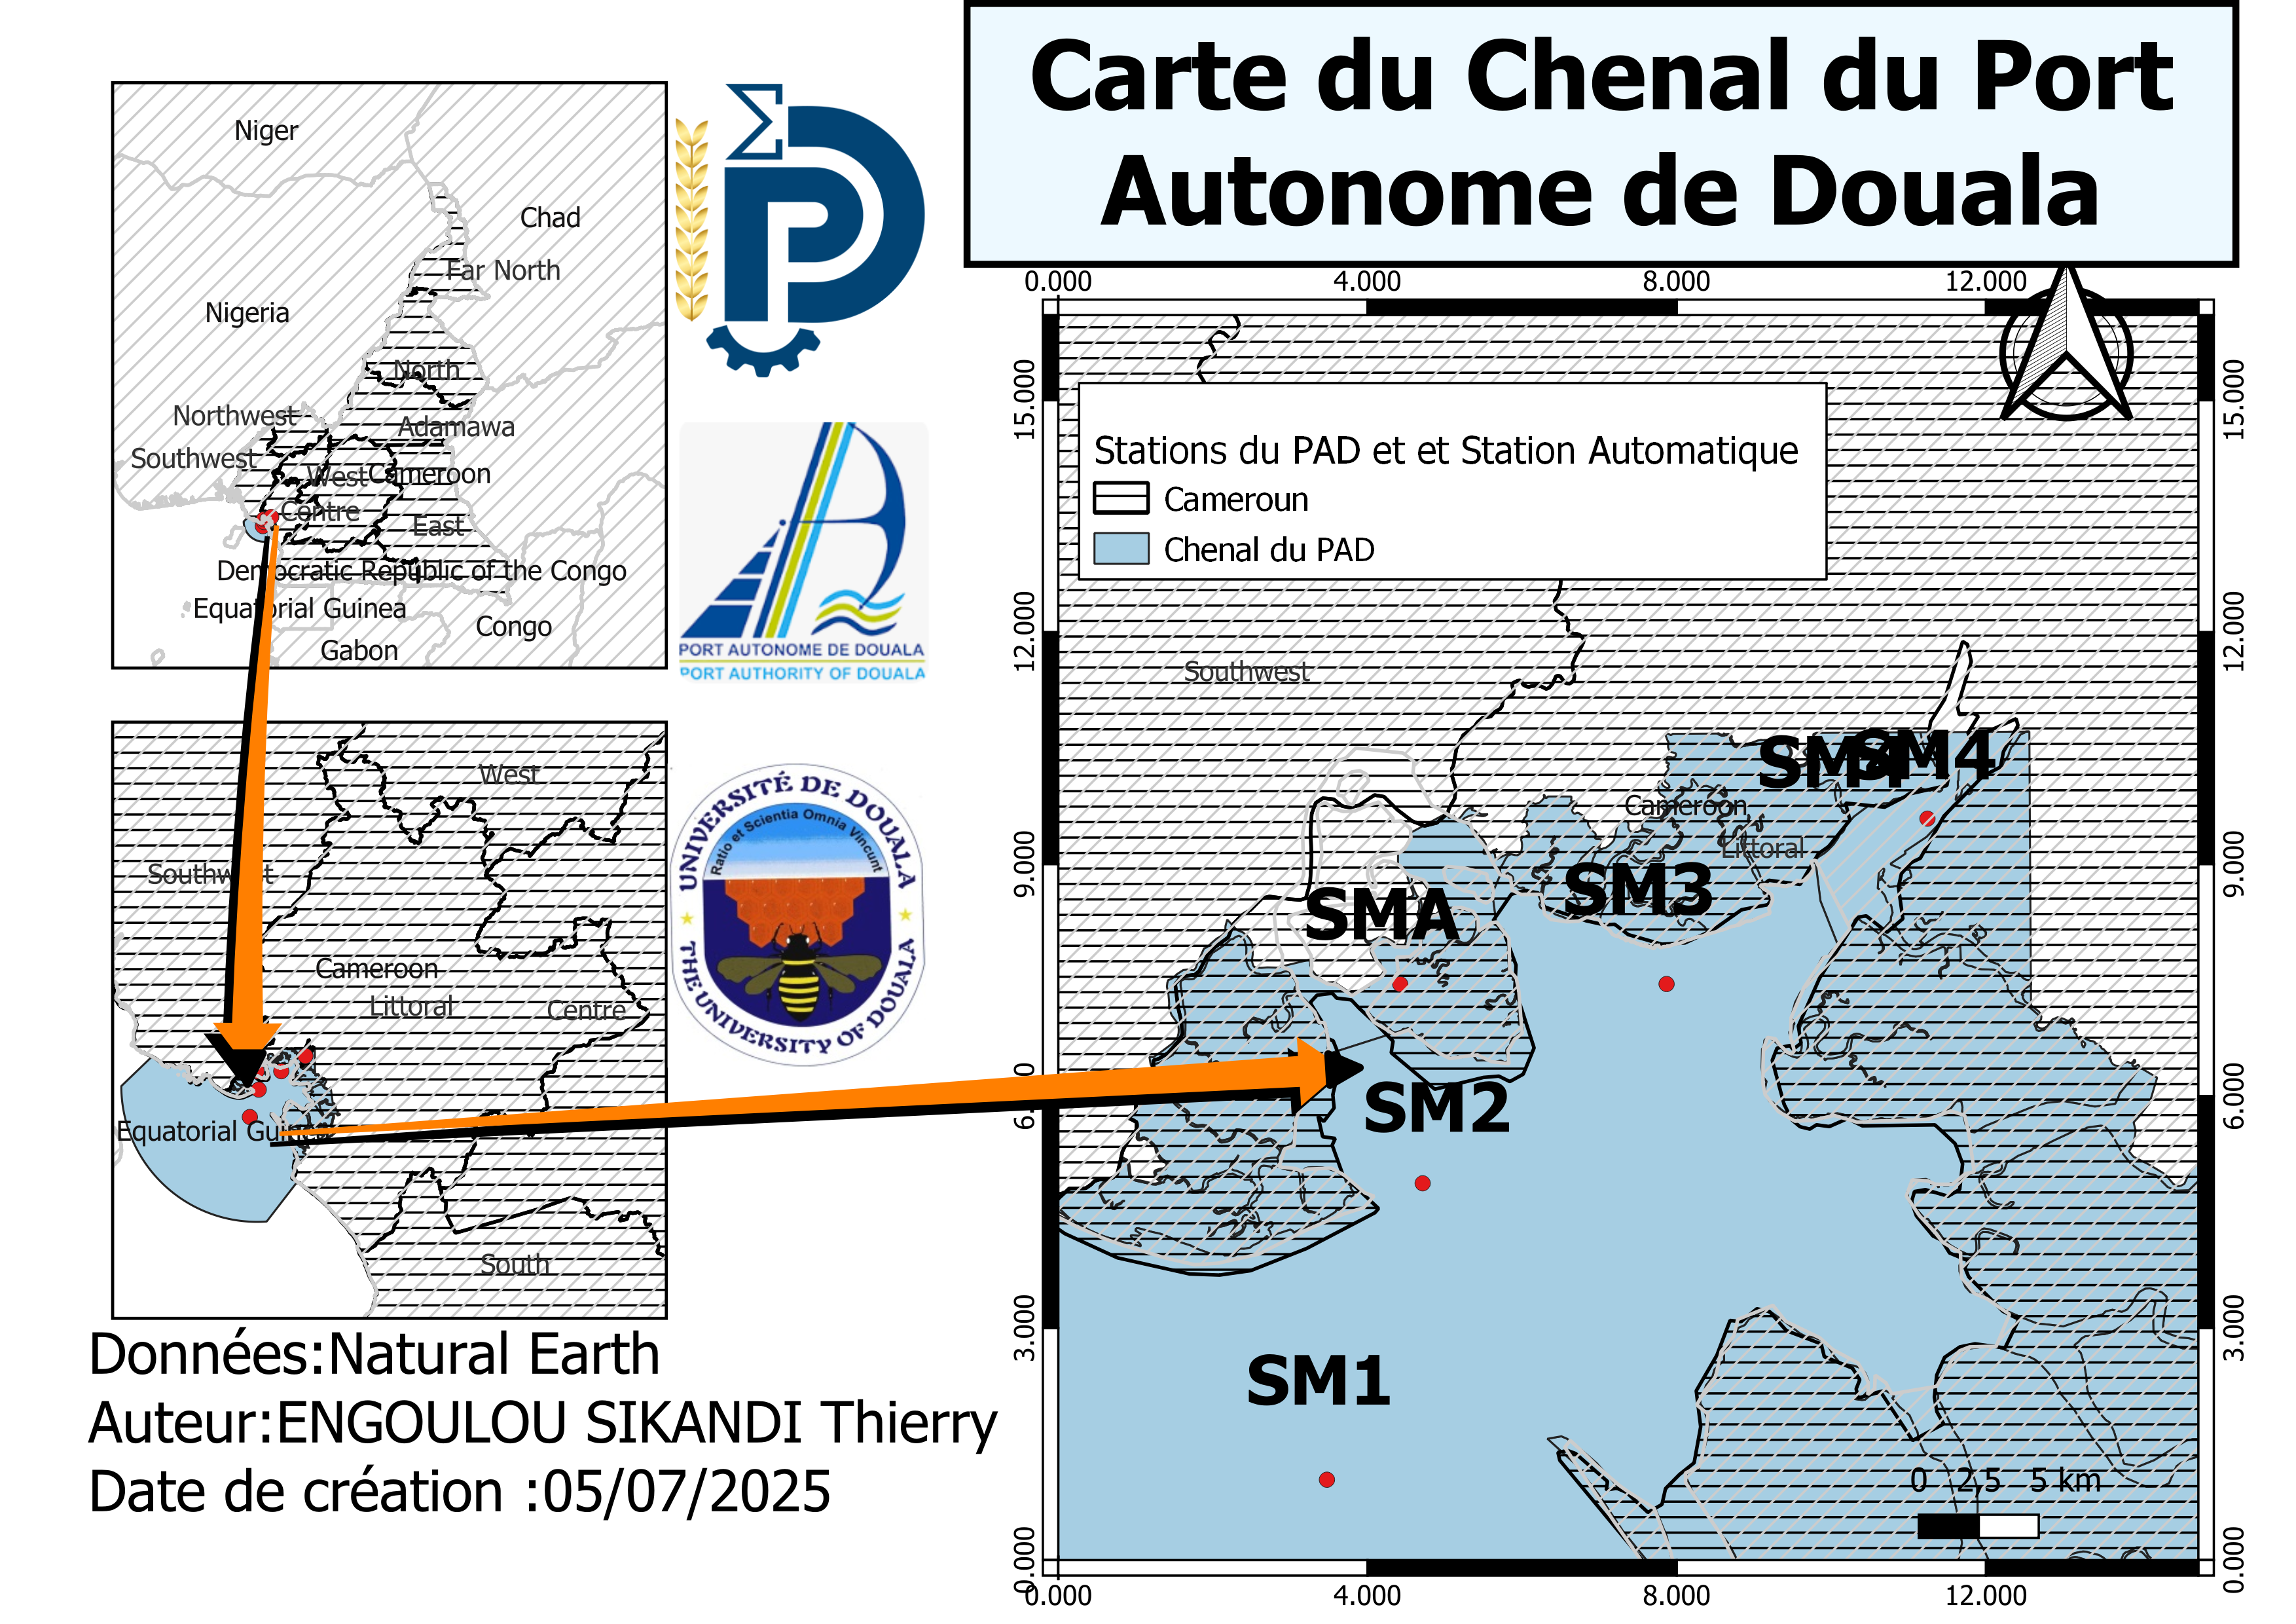
\includegraphics[width=1\textwidth,height=4in]{images/Zone_E_PAD_Vrai.png}
	    	      \end{center}
	    	     \end{minipage}

					\caption{Zone d'étude \label{Fig 2.1} } 
		\end{center}
	\end{figure}


\quad
	Par ailleurs, les équipements portuaires sont particulièrement sensibles aux vents forts, averses tropicales et aux tempêtes locales souvent intenses en saison des pluies . Une prévision fiable de ces phénomènes permet de renforcer les mesures de sécurité, notamment pour les grues,
	 les conteneurs et les opérations de déchargement.
	 
	\subsection{Rôle du port dans les conditions météorologiques nationales}
	En tant que point stratégique d’échanges économiques, le Port de Douala joue un rôle central dans la régulation des conditions météorologiques locales avec des effets d’amplification à l’échelle régionale. Il constitue un hub d’observation pour plusieurs réseaux météorologiques (Météo Cameroun, Université de Douala, ...) qui alimentent les systèmes nationaux de veille climatique.
	Son positionnement sur le littoral camerounais en fait un point de référence météorologique national, notamment pour :\\
\begin{itemize}
	\item Le suivi des cyclones tropicaux et orages côtiers,\\
	\item La prévision des marées pour la navigation fluviale et maritime,\\
	\item La collecte de données atmosphériques utiles à la modélisation du climat national.\\
\end{itemize}

\quad	Les données issues de ses capteurs sont cruciales pour l’alerte précoce en cas d’événements extrêmes, la planification portuaire, mais aussi la calibration de modèles climatiques régionaux utilisés par les agences nationales et partenaires internationaux.

	\section{Présentation des équipements météorologiques et maréographiques du PAD}
	
	\quad
	Le Port Autonome de Douala , compte tenu de sa position géographique stratégique et de son rôle dans le commerce maritime national, a mis en place un ensemble d’équipements scientifiques pour surveiller les conditions environnementales. Ces dispositifs permettent une acquisition en temps réel de paramètres météorologiques et maréographiques essentiels à la navigation, à la sécurité portuaire et à la planification logistique.
	Ces instruments sont installés sur différents sites du port et sont exploités par plusieurs entités, notamment Météo Cameroun, le Service hydrographique du PAD et des partenaires techniques comme l’Université de Douala. L’automatisation et la télémesure permettent une transmission continue des données vers des plateformes locales .
		\subsection{Équipements météorologiques}
		
		\quad Les équipements météorologiques du Port Autonome de Douala comprennent des stations autonomes capables de mesurer en continu divers paramètres atmosphériques tels que la température, l'humidité,le point de rosée , la pression, la direction et la vitesse du vent,...  ainsi que des capteurs fixés sur des bouées ou infrastructures portuaires(SM1 ,SM2 ,SM3, et SM4). Ces dispositifs sont conçus pour fonctionner en environnement marin et transmettre automatiquement les données collectées à une base centrale par réseau  radio(TideMaster).Ces données sont ensuite stockées,   mises à disposition en temps réel via une interface numérique pour les utilisateurs du port.Ce système est renforcé par un partenariat technique avec la Direction de la Météorologie Nationale  , qui accompagne le PAD dans l’entretien des équipements, l’exploitation conjointe des données et l’élaboration de bulletins météo spécialisés. L’ensemble vise à améliorer la sécurité maritime, anticiper les risques climatiques et faciliter la prise de décision pour les activités portuaires et logistiques pour une illustration voir figure \ref{Fig 2.2}. \\
		
			\subsubsection{Équipements maréographiques}
			
			\quad Les stations marégraphiques fonctionnent en mesurant le niveau de la mer de manière continue, à l’aide de capteurs très précis installés sur des quais ou des structures flottantes. Ces capteurs peuvent être de différents types : à flotteur  , à pression  , radar ou encore acoustique  . Les mesures sont enregistrées à intervalles réguliers par une unité d’acquisition(10 minutes), puis stockées   transmises vers un un database local via radiofréquence.Au Port Autonome de Douala, ces stations permettent une surveillance continue du niveau marin afin de sécuriser les activités portuaires, notamment les opérations d’accostage et de navigation. En plus de leur rôle opérationnel, elles fournissent des séries de données cruciales pour la modélisation hydrodynamique, les études d’aménagement côtier et la prévision des marées pour une illustration voir figure \ref{Fig 2.3}.
			\begin{figure}[H]
			\begin{center}
                \begin{minipage}{\textwidth}
	    	     \begin{center}
	    	      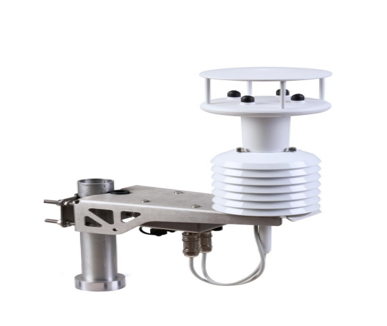
\includegraphics[width=1\textwidth,height=4.6in]{images/Station_meteo_pad.png}
	    	      \end{center}
	    	     \end{minipage}
					
					
					\caption{Station météorologiaue du PAD\label{Fig 2.2}}
				\end{center}
			\end{figure}	
		
	\subsection{Presentation , fonctionnement et système d’acquisition de données  des  stations du PAD}

\quad Les stations installées autour du Port Autonome de Douala génèrent des donnnées,La collecte des données météorologiques repose sur deux sources principales : les stations du Port Autonome de Douala (notamment SM2, SM3, et SM4), via radio frequence et ces données sont stocker en fichier tex .Les Graphiques temps réel (température, niveau de la mer, vent, etc.) via dashboar sont en partie visible sur la  Figure \ref{Fig 2.5} .
\section{Système de gestion et de visualisation des données}
		\begin{figure}[H]
			\begin{center}
                \begin{minipage}{\textwidth}
	    	     \begin{center}
	    	      \includegraphics[width=1\textwidth,height=4.6in]{images/marégraphe.png}
	    	      \end{center}
	    	     \end{minipage}
				
				
				\caption{Station marégrapique du PAD \label{Fig 2.3}}
			\end{center}
		\end{figure}%
	
		
		\subsection{Collecte des données}
		
		\quad Le système d’acquisition de données mis en place dans le cadre de ce projet repose sur un chaînage technologique automatisé, combinant la collecte, la transmission, le stockage et la visualization local  des données environnementales issues du Port Autonome de Douala via cloud. Ce système est fondé sur une approche temps réel, modulaire et évolutive, intégrant des composants open source et des solutions cloud pour faciliter la prévision et l’analyse continue. En effet, certaines stations du port ne capturent pas encore toutes les variables nécessaires pour l'entraînement d’un modèle complet, en particulier les précipitations. C’est pourquoi une station de substitution située à Akwa, proche du port, a été intégrée via OpenWeatherMap pour garantir la disponibilité des cibles (targets) du modèle voir Figure \ref{Fig 2.4}.
		
	\begin{figure}[H]
	\begin{center}
                \begin{minipage}{\textwidth}
	    	     \begin{center}
	    	      \includegraphics[width=1\textwidth,height=4.6in]{images/système_aquisition_data_PAD.png}
	    	      \end{center}
	    	     \end{minipage}
		
		
		\caption{Système d'acquisition des données au PAD \label{Fig 2.4}}
	\end{center}
\end{figure}%	

	\subsection{Plateforme de stockage}

\quad Les données collectées sont centralisées dans une base de données MongoDB et dans un fichier exell , accessible à distance via une API REST développée avec Flask. Cette API permet de requêter les observations récentes par station, par date, ou selon une limite spécifiée. Elle facilite l'intégration des données dans d'autres systèmes, y compris dans les interfaces de visualisation web. Pour la robustesse et l’accessibilité, cette API est hébergée sur la plateforme Render voir figure \ref{Fig 2.4}.


\subsection{Visualisation des données}

\quad Les données sont affichées dynamiquement sur une interface développée avec Streamlit et react  (voir le site). Elle présente les dernières observations des stations (SM2, SM3, SM4 et station externe), affiche des graphes temporels par station et paramètre, et fournit une carte interactive alimentée par Folium et Plotly sans oublier les previsions météorologique . Un iframe Windy et copernicus  sont  également intégrés pour enrichir l’expérience utilisateur avec des prévisions animées en temps réel voir figure \ref{Fig 2.5}.

	\begin{figure}[H]
	\begin{center}
      \begin{minipage}{\textwidth}
	   \begin{center}
	   \includegraphics[width=1\textwidth,height=4.6in]{images/système_acquisition.png}
	   \end{center}
	   \end{minipage}
		
		
		\caption{Visualisation locale des données du PAD \label{Fig 2.5} }
	\end{center}
\end{figure}%	



	
	\subsection{Présentation des variables  utilisées}
	\quad Les variables utilisées incluent la température de l’air, l’humidité, la vitesse du vent, la pression atmosphérique,direction du vent , précipitation ,la hauteur de marée (TIDE HEIGHT) et le SURGE. Ces données ont été collectées sur une période suffisante pour entraîner des modèles de prévision. Les fichiers sources sont sauvegardés dans des formats Excel, puis traités automatiquement via des scripts Python.
	Comprendre l'architetecture de notre travail cf Figure\ref{Fig 2.6} 
			\begin{figure}[H]
		\begin{center}
			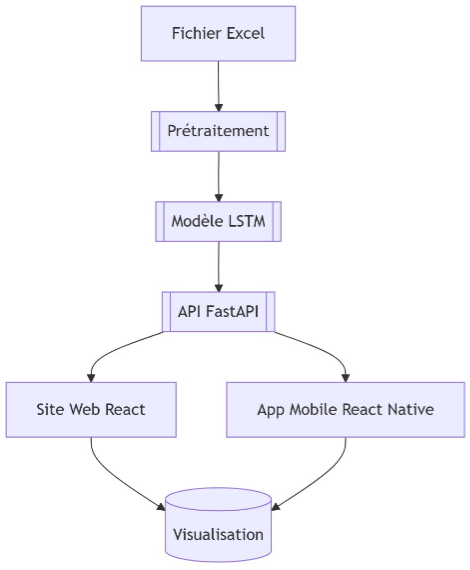
\includegraphics[scale=0.59]{images/Travail.png}
			\caption{\emph{	Architecture de notre travail }\label{Fig 2.6}} %\label{fig:1}
		\end{center}
	\end{figure}
	
	\section{Modélisation prédictive des données}
	
	\subsection{Filtrage des données}
	
	\quad Un premier nettoyage est effectué pour retirer les colonnes non numériques ou mal formatées. Les chaînes de caractères, coordonnées géographiques, et dates sont converties ou supprimées lorsque non exploitables. Cette étape est primordiale pour s’assurer que les modèles reçoivent uniquement des données valides.
	\subsection{Prétraitement des données}
	
	\quad Un script dédié (data\_preprocessing.py) assure le traitement des séries temporelles : normalisation (MinMaxScaler), découpage en séquences (time\_steps variant entre 10 et 20), création des jeux de données d’entraînement et de test. Les scalers sont sauvegardés pour une réutilisation cohérente lors de l’inférence.

	\quad Le modèle choisi est un LSTM multivarié, implémenté avec Keras. Il comprend plusieurs couches LSTM empilées et des mécanismes de régularisation (Dropout, EarlyStopping). L’objectif est de prédire la température et les précipitations sur un horizon de 7 jours. Le modèle est entraîné sur les données des stations (SM2, SM3, SM4 et Akwa).
	\subsection{Validation du modele}
	
	\quad La validation du modèle LSTM s’inscrit dans une approche rigoureuse tenant compte de la nature séquentielle des données météorologiques. Contrairement aux modèles classiques, il est impératif de conserver l’ordre chronologique lors de la division du jeu de données. Les données les plus anciennes sont utilisées pour l’entraînement, une période intermédiaire pour la validation, et enfin, les données les plus récentes pour le test final.
	
	 Cette séparation temporelle prévient les fuites d’information et reflète mieux le comportement réel du modèle face à des situations futures non vues durant l’apprentissage.Afin d’évaluer la stabilité du modèle dans le temps, une stratégie de validation croisée adaptée aux séries temporelles a été mise en œuvre, notamment la validation glissante (walk-forward validation). Elle consiste à entraîner le modèle sur une première fenêtre temporelle, puis à le tester sur la période suivante. Cette fenêtre est ensuite déplacée progressivement, ce qui permet d’observer la robustesse du modèle sur différents segments temporels. Ce procédé offre une meilleure représentativité des performances que la validation classique aléatoire, qui n’est pas adaptée aux dépendances temporelles.\\
	Les performances du modèle LSTM ont été suivies à l’aide de trois métriques complémentaires : MAE, RMSE et MAPE. Le MAE indique l’erreur moyenne quotidienne, tandis que le RMSE met en lumière les erreurs plus importantes, utiles pour détecter les épisodes extrêmes mal anticipés. Le MAPE, exprimé en pourcentage, facilite quant à lui la comparaison entre stations ou périodes, bien qu’il puisse être instable lors de faibles précipitations. L’utilisation combinée de ces métriques permet donc une évaluation fine, à la fois absolue, relative et sensible aux écarts majeurs, confirmant ainsi la pertinence du modèle tout en révélant des pistes d’amélioration.\\
	
	\subsection{Métriques d'évaluation des modèles de régression}
	
	\textbf{Le coefficient de détermination est défini par }:
	
	\begin{equation}
		R^2 = 1 - \frac{\sum_{i=1}^{n} (y_i - \hat{y}_i)^2}{\sum_{i=1}^{n} (y_i - \bar{y})^2}  ,
	\end{equation}
	
	où $y_i$ représente la valeur observée, $\hat{y}_i$ la valeur prédite par le modèle, et $\bar{y}$ la moyenne des valeurs observées. Le numérateur correspond à la somme des carrés des résidus (erreur du modèle), et le dénominateur à la somme totale des carrés (variabilité totale). Ainsi, $R^2$ mesure la proportion de la variance expliquée par le modèle. Une valeur proche de 1 indique un bon ajustement.
	
	\vspace{1em}
	
	\noindent \textbf{Erreur Absolue Moyenne (MAE)} :
	\begin{equation}
		\text{MAE} = \frac{1}{n} \sum_{i=1}^{n} \left| y_i - \hat{y}_i \right|          .
	\end{equation}
	
	La MAE estime l'erreur absolue moyenne entre les valeurs réelles et les prédictions. Elle exprime directement, dans l’unité de la variable cible, l’écart typique que le modèle commet au quotidien. Elle est simple à interpréter et moins sensible aux valeurs extrêmes.
	
	\vspace{1em}
	
	\noindent \textbf{Racine de l’Erreur Quadratique Moyenne (RMSE)} :
	\begin{equation}
		\text{RMSE} = \sqrt{ \frac{1}{n} \sum_{i=1}^{n} (y_i - \hat{y}_i)^2 }      .
	\end{equation}
	
	La RMSE pénalise plus fortement les grandes erreurs que la MAE en élevant les écarts au carré. Elle met donc davantage en évidence les épisodes où le modèle sous-performe fortement, ce qui est pertinent pour des phénomènes comme les fortes précipitations.
	
	\vspace{1em}
	
	\noindent \textbf{Erreur Moyenne Absolue en Pourcentage (MAPE)} :
	\begin{equation}
		\text{MAPE} = \frac{100}{n} \sum_{i=1}^{n} \left| \frac{y_i - \hat{y}_i}{y_i}  . \right|                  .
	\end{equation}
	
	Le MAPE exprime l’erreur moyenne en pourcentage relatif par rapport aux valeurs réelles. Cela facilite la comparaison entre périodes ou entre stations, mais cette métrique peut être instable si certaines valeurs observées $y_i$ sont très proches de zéro.
	

	\section{Développement du site de visualisation}

	\subsection{Plateforme de visualisation des données et prévisions en temps réel}
	
	\quad Le site web développé avec Streamlit et react propose une visualisation interactive des paramètres météo. Il contient :\\
	\begin{enumerate}
		\item Une carte \textbf{Folium} avec les stations géolocalisées,\\
		\item Des graphiques dynamiques par station/paramètre,\\
		\item Une mini-carte animée \textbf{Windy} pour le vent,\\
		\item Une interface de téléchargement \textbf{CSV}.
	\end{enumerate}
	Une section supplémentaire est prévue pour afficher chaque matin les prévisions météorologiques  basées sur le modèle LSTM ainsi que sur les données externes (WRF, Windy, Copernicus,...).
		
	
	\newpage
	\section*{}
	
	\quad Le Ce chapitre a permis de décrire en détail l’architecture technique et méthodologique mise en place pour la prévision météorologique et marégraphique à Douala. À travers l’intégration des données issues des stations SM2, SM3 et SM4 du Port Autonome de Douala, complétées par des sources externes fiables comme OpenWeatherMap, un système robuste d’acquisition, de traitement et de visualisation des données a été établi.La modélisation prédictive basée sur les réseaux de neurones LSTM permet de fournir des prévisions multivariées , avec des performances validées selon plusieurs métriques. En parallèle, un site web interactif a été développé pour la diffusion en temps réel des données et des prévisions, appuyé par une infrastructure cloud (Render, MongoDB ,google sheets) garantissant l’accessibilité à distance.Malgré certaines limitations matérielles (capteurs incomplets) et logicielles (conexion internet et l'automatisation du modèle des marées ), cette approche constitue une base innovante et évolutive pour la surveillance météorologique locale. Elle ouvre également des perspectives d’intégration de prévisions plus avancées via des outils comme WRF, Windy ou Copernicus.
	
%======================================================================================================================= %	
	\chapter{RÉSULTATS ET DISCUSSION}
	\label{ch:résultatsetdiscussion} %\thispagestyle{empty} 
%	\clearpage
%	\newpage
%	

%	
\section*{}
\quad Dans ce chapitre, nous présentons l'ensemble du processus pratique mis en œuvre pour la réalisation du système de prévision météorologique et marégraphique à Douala puis précisement aux Port Autonome de Douala. Cette phase intègre l'entraînement du modèle LSTM, l'évaluation de ses performances, la conception de l’interface web de visualisation ainsi que le déploiement de l’application sur le web. L'objectif final est de proposer un outil accessible, capable de fournir quotidiennement des prévisions fiables généré par un prévisioniste en s’appuyant à la fois sur les données collectées localement et sur des ressources numériques avancées
%	\newpage

\section{Modélisation avec LSTM}

\subsection{Entraînement du modèle prédictif}

\quad L'entraînement du modèle s’est basé sur les données météorologiques multivariées collectées auprès des stations SM2, SM3 et SM4 du Port Autonome de Douala, complétées par les données issues d’OpenWeatherMap pour les précipitations. Le modèle est un réseau LSTM multivarié construit avec Keras et TensorFlow. Après un prétraitement rigoureux (nettoyage, normalisation et séquençage), les données ont été divisées en ensembles d’apprentissage (80 \%) et de test (20 \%).
Différents time\_steps ont été testés (10, 15, 20) pour déterminer la meilleure fenêtre temporelle pour la prédiction. Le modèle a été entraîné pour prédire deux cibles : la température et les précipitations, sur un horizon de sept jours. Un EarlyStopping a été utilisé pour éviter l’overfitting ,le resultat est affiché sur la Figure \ref{Fig 3.1}.

\begin{figure}[H]
	\begin{center}
		 \begin{minipage}{\textwidth}
		    \begin{center}
		    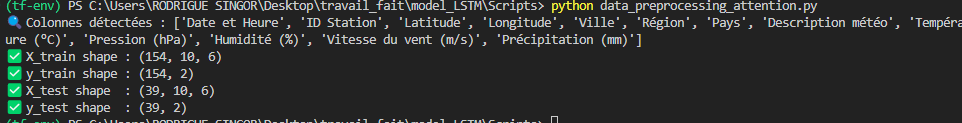
\includegraphics[width=1\textwidth,height=2in]{images/TRAITEMENT_TEXT.png}
		    \end{center}
		    \end{minipage}
		\caption{Sortie de du traitement et du test du modèle \label{Fig 3.1}}
	\end{center}
\end{figure}

\subsection{Résultats de la prédiction avec LSTM}



	\begin{figure}[H]
	\begin{center}
		 \begin{minipage}{\textwidth}
		    \begin{center}
		    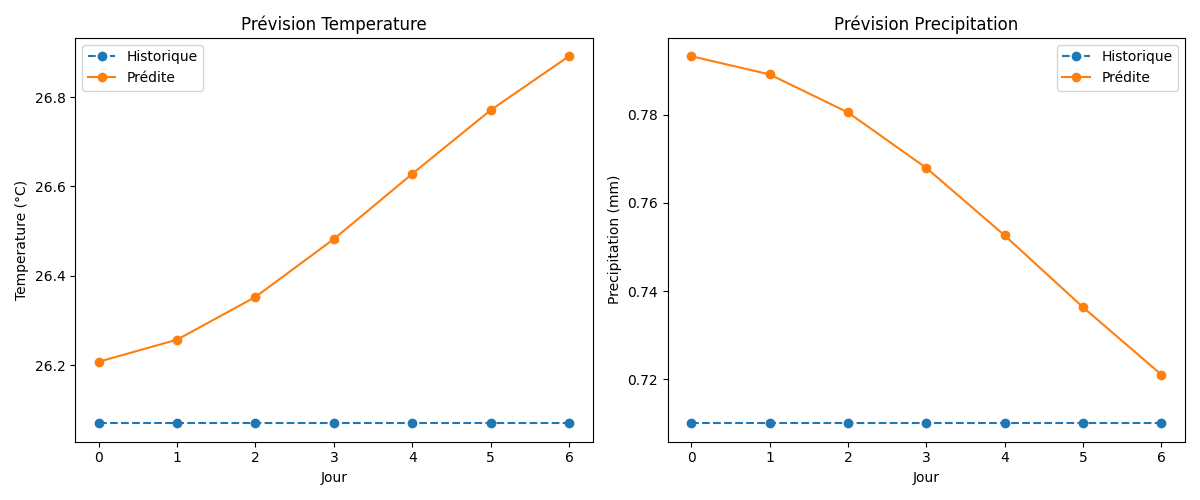
\includegraphics[width=1\textwidth,height=4.3in]{images/time_steps10_vraiF.png}
		    \end{center}
		    \end{minipage}
		
		
		\caption{Sortie du 1er time\_steps \label{Fig 3.2}}
	\end{center}
\end{figure}%	score_LSTM-T
\begin{figure}[H]
	\begin{center}
		 \begin{minipage}{\textwidth}
		    \begin{center}
		    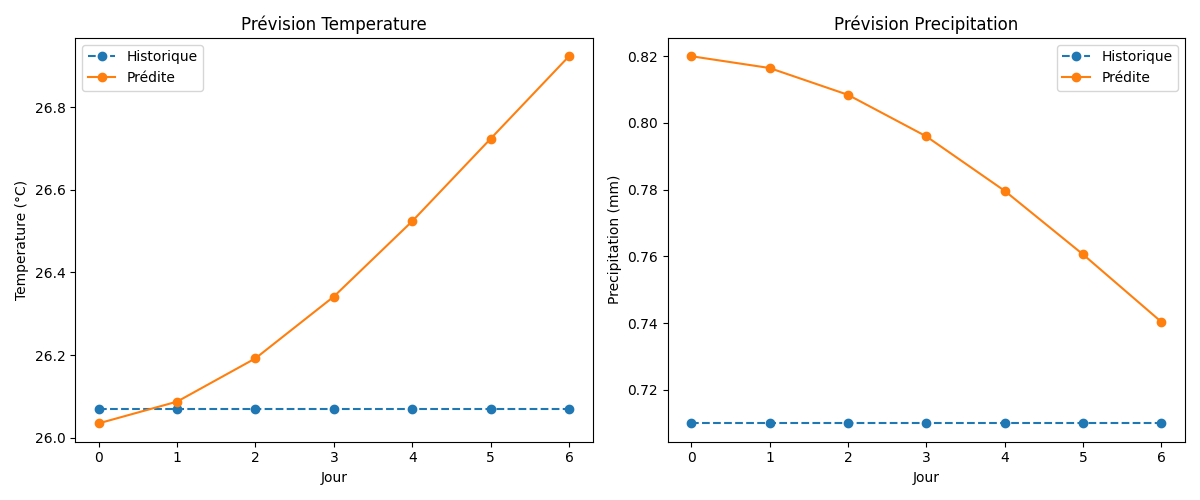
\includegraphics[width=1\textwidth,height=4.6in]{images/Time_steps15_F.png}
		    \end{center}
		    \end{minipage}
	\caption{Sortie du 2ième time\_steps \label{Fig 3.3}}
	
	
		\subsection{Analyse des Résultats  }
		
		
		\quad
		
		
		\begin{center}
					Le modèle LSTM prédit, pour les jours 0 à 6 selon les figures \ref{Fig 3.2},\ref{Fig 3.2},\ref{Fig 3.3} nous montre une \textbf{hausse progressive de la température} pour les 3 pas de temps, allant d’environ 26{,}04\,°C à 26{,}92\,°C, ainsi qu’une \textbf{baisse régulière des précipitations}, de 0{,}82\,mm à 0{,}74\,mm. Ces variations contrastent avec les valeurs historiques quasiment constantes (~26{,}07\,°C et ~0{,}71\,mm), ce qui indique que le modèle ne se contente pas d’une moyenne stationnaire, mais parvient à capturer des \textbf{tendances temporelles}, un réchauffement modéré (+0{,}88\,°C) et une baisse des précipitations (–0{,}08\,mm) sur une semaine. Ce comportement illustre la capacité des réseaux LSTM à modéliser les \emph{dépendances séquentielles} dans les séries temporelles.Par ailleurs, l’évaluation de la qualité des prédictions repose sur l’analyse de métriques d’erreur telles que la \emph{Mean Absolute Error (MAE)} et la \emph{Root Mean Square Error (RMSE)}. La MAE mesure l’erreur moyenne absolue, offrant une interprétation directe en unité de mesure (°C ou mm), tandis que la RMSE accorde un poids plus important aux erreurs importantes, ce qui permet de détecter les fluctuations mal anticipées par le modèle.
			
		\end{center}

		
	
	\end{center}
\end{figure}%	


\begin{figure}[H]
\begin{center}
		 \begin{minipage}{\textwidth}
		    \begin{center}
		    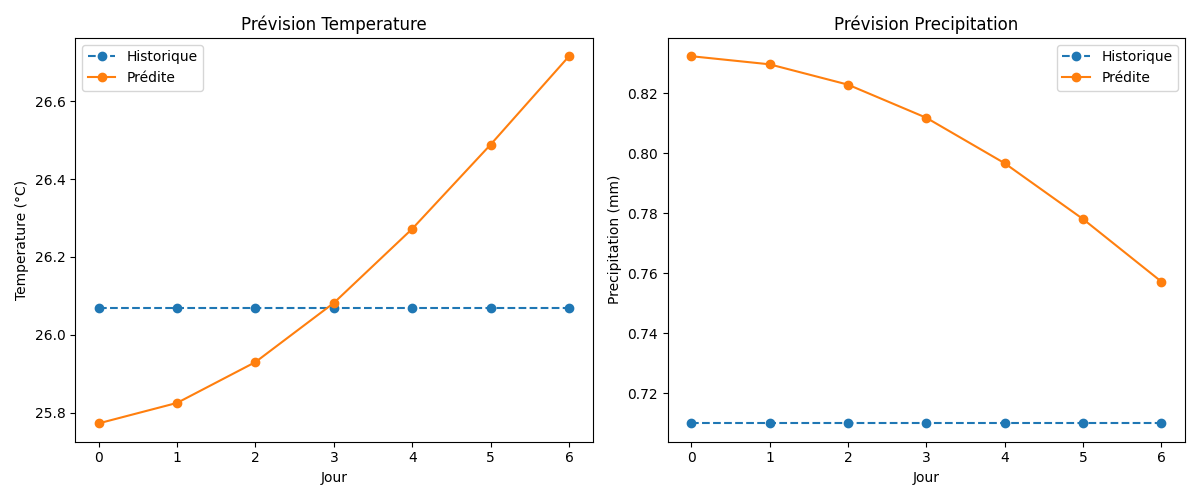
\includegraphics[width=1\textwidth,height=4.3in]{images/time_steps20_vraiF.png}
		    \end{center}
		    \end{minipage}

	
	\caption{Sortie du 3ième time\_steps\label{Fig 3.4}}
\end{center}
\end{figure}%	


	




\section{Validation du modèle LSMT  }
		\subsection{Justification méthodologique de la comparaison}
	
	\quad
	Dans le cadre de la prévision météorologique appliquée aux opérations portuaires, la validation d’un modèle avancé tel que le \textbf{LSTM} doit s’appuyer sur une comparaison rigoureuse avec des modèles de référence bien établis. Deux approches classiques ont été sélectionnées à cet effet : le \textbf{modèle de persistance} et le \textbf{modèle ARIMA}. Le modèle de persistance, souvent utilisé comme \textit{baseline} minimaliste, repose sur une hypothèse intuitive : la valeur future est identique à la dernière observation connue. Ce modèle, bien que rudimentaire, est réputé pour son efficacité à court terme, notamment pour des variables comme la température qui présentent une forte inertie temporelle.
	
	À l’opposé, le modèle ARIMA, largement reconnu dans la littérature en météorologie, permet de modéliser les dépendances linéaires dans les séries temporelles avec une relative simplicité computationnelle. En les intégrant comme points de comparaison, cette étude assure un ancrage méthodologique solide et transparent, permettant d’évaluer objectivement les apports du LSTM.
	
	\subsection{Analyse des performances comparatives}
	
	\quad
	Les performances observées mettent en évidence la supériorité globale du modèle LSTM, en particulier pour la variable \textbf{Température}. \textbf{Le modèle LSTM} enregistre la meilleure erreur absolue moyenne (\textbf{MAE} : 0{,}63~°C) et la meilleure erreur quadratique moyenne (\textbf{RMSE} : 0{,}84~°C), surpassant nettement les scores obtenus par ARIMA (MAE : 2{,}29~°C) et par le modèle de persistance (MAE : 1{,}67~°C). Cette performance traduit une meilleure aptitude à capturer des dynamiques complexes et non linéaires, caractéristiques des phénomènes météorologiques.
	
	En ce qui concerne la \textbf{Précipitation}, le modèle ARIMA obtient un MAE plus faible (0{,}36~mm), mais son instabilité en \textbf{MAPE} le rend peu interprétable dans ce contexte. Le LSTM, quant à lui, maintient une cohérence et une régularité des erreurs, ce qui le rend plus robuste, notamment face à la forte variabilité et à la nature sporadique des précipitations. Ces constats sont renforcés par le \textit{barplot} généré, qui visualise clairement l’avantage du LSTM sur les deux métriques retenues cf Tableau\ref{tab:resultats_mae_rmse} et \ref{tab:comparison_models}.
	\begin{center}
		\begin{table}
		\caption{Erreurs MAE et RMSE par modèle pour les deux variables étudiées}
		Tableau 3.0-Erreurs MAE et RMSE par modèle pour les deux variables étudiées
		
		\begin{tabular}{|l|l|c|c|}
			\hline
			\textbf{Modèle} & \textbf{Variable} & \textbf{MAE} & \textbf{RMSE} \\
			\hline
			LSTM & Température (°C)   & 0{,}63 & 0{,}84 \\
			\hline
			ARIMA & Température (°C)  & 2{,}29 & 2{,}49 \\
			\hline
			Persistance & Température (°C) & 1{,}67 & 1{,}80 \\
			\hline
			\hline
			LSTM & Précipitation (mm) & 0{,}94 & 1{,}38 \\
			\hline
			ARIMA & Précipitation (mm) & 0{,}36 & 0{,}41 \\
			\hline
			Persistance & Précipitation (mm) & 1{,}11 & 1{,}50 \\
			\hline
		\end{tabular}
		\label{tab:resultats_mae_rmse}
	\end{table}
	\end{center}
	%		
	
	\subsection{Choix justifié du modèle LSTM}
	
	\begin{table}[H]
		\centering
		\caption{Comparaison des performances des modèles CNN 1D, LSTM et BiLSTM}
		\begin{tabular}{|l|c|c|c|c|}
			\toprule
			\textbf{Modèle} & \textbf{MSE} & \textbf{MAE} & \textbf{RMSE} & \textbf{R\textsuperscript{2}} \\
			\midrule
			CNN 1D  & 0.4 & 0.4 & 0.6 & 0.6 \\
			\hline
			LSTM    & 0.4 & 0.4 & 0.6 & 0.6 \\
			\hline
			BiLSTM  & 0.4 & 0.4 & 0.6 & 0.6 \\
			\bottomrule
		\end{tabular}
		\label{tab:comparison_models}
	\end{table}
	\begin{figure}[H]
		\begin{center}
		 \begin{minipage}{\textwidth}
		    \begin{center}
		    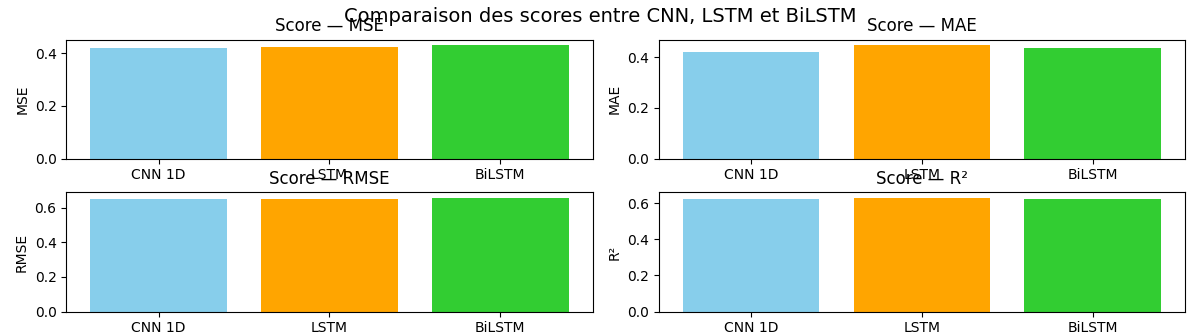
\includegraphics[width=1\textwidth,height=4in]{images/3_SCORE.png}
		    \end{center}
		    \end{minipage}

			\caption{Comparaison des modeles D'IA\label{Fig 3.5}}
		\end{center}
	\end{figure}
	
	\subsection{Analyse des performances}
	
	Selon la Figure \ref{Fig 3.5} ,les résultats obtenus montrent que les trois modèles\textbf{CNN 1D}, \textbf{LSTM} et \textbf{BiLSTM} présentent des performances \emph{quasi identiques} sur le jeu de données météorologiques utilisé, avec un MSE de 0{,}4, un MAE de 0{,}4, un RMSE de 0{,}6 et un coefficient de détermination \( R^2 \) de 0{,}6. Cette similarité peut s’expliquer par la nature du jeu de données (peu bruité ou faiblement non linéaire), ou par des paramètres d'entraînement communs. Cela suggère que des modèles \textbf{plus simples comme le CNN 1D} peuvent suffire dans certains cas, sans nécessairement recourir à la complexité computationnelle du BiLSTM. Toutefois, une évaluation sur des données plus complexes ou à plus grande échelle permettrait de mieux distinguer les forces de chaque architecture.\\
	Compte tenu de la structure complexe et potentiellement chaotique des données météorologiques, le recours au \textbf{LSTM} apparaît pleinement justifié. Son architecture à mémoire récurrente lui permet d’apprendre des séquences temporelles longues, d’anticiper les tendances saisonnières et d’atténuer l’impact des fluctuations aléatoires, là où ARIMA et Persistance restent limités par leurs fondements linéaires ou naïfs cf Figure\ref{Fig 3.6}.
	
	Bien qu’exigeant en ressources pour l’entraînement, le modèle LSTM a démontré une valeur prédictive tangible et une généralisation plus robuste sur les deux variables étudiées. Il s’impose donc comme la solution la plus adaptée pour des prévisions à la fois précises et résilientes dans un environnement portuaire exposé à des aléas météorologiques complexes.
	\begin{figure}[H]
		\begin{center}
		 \begin{minipage}{\textwidth}
		    \begin{center}
		    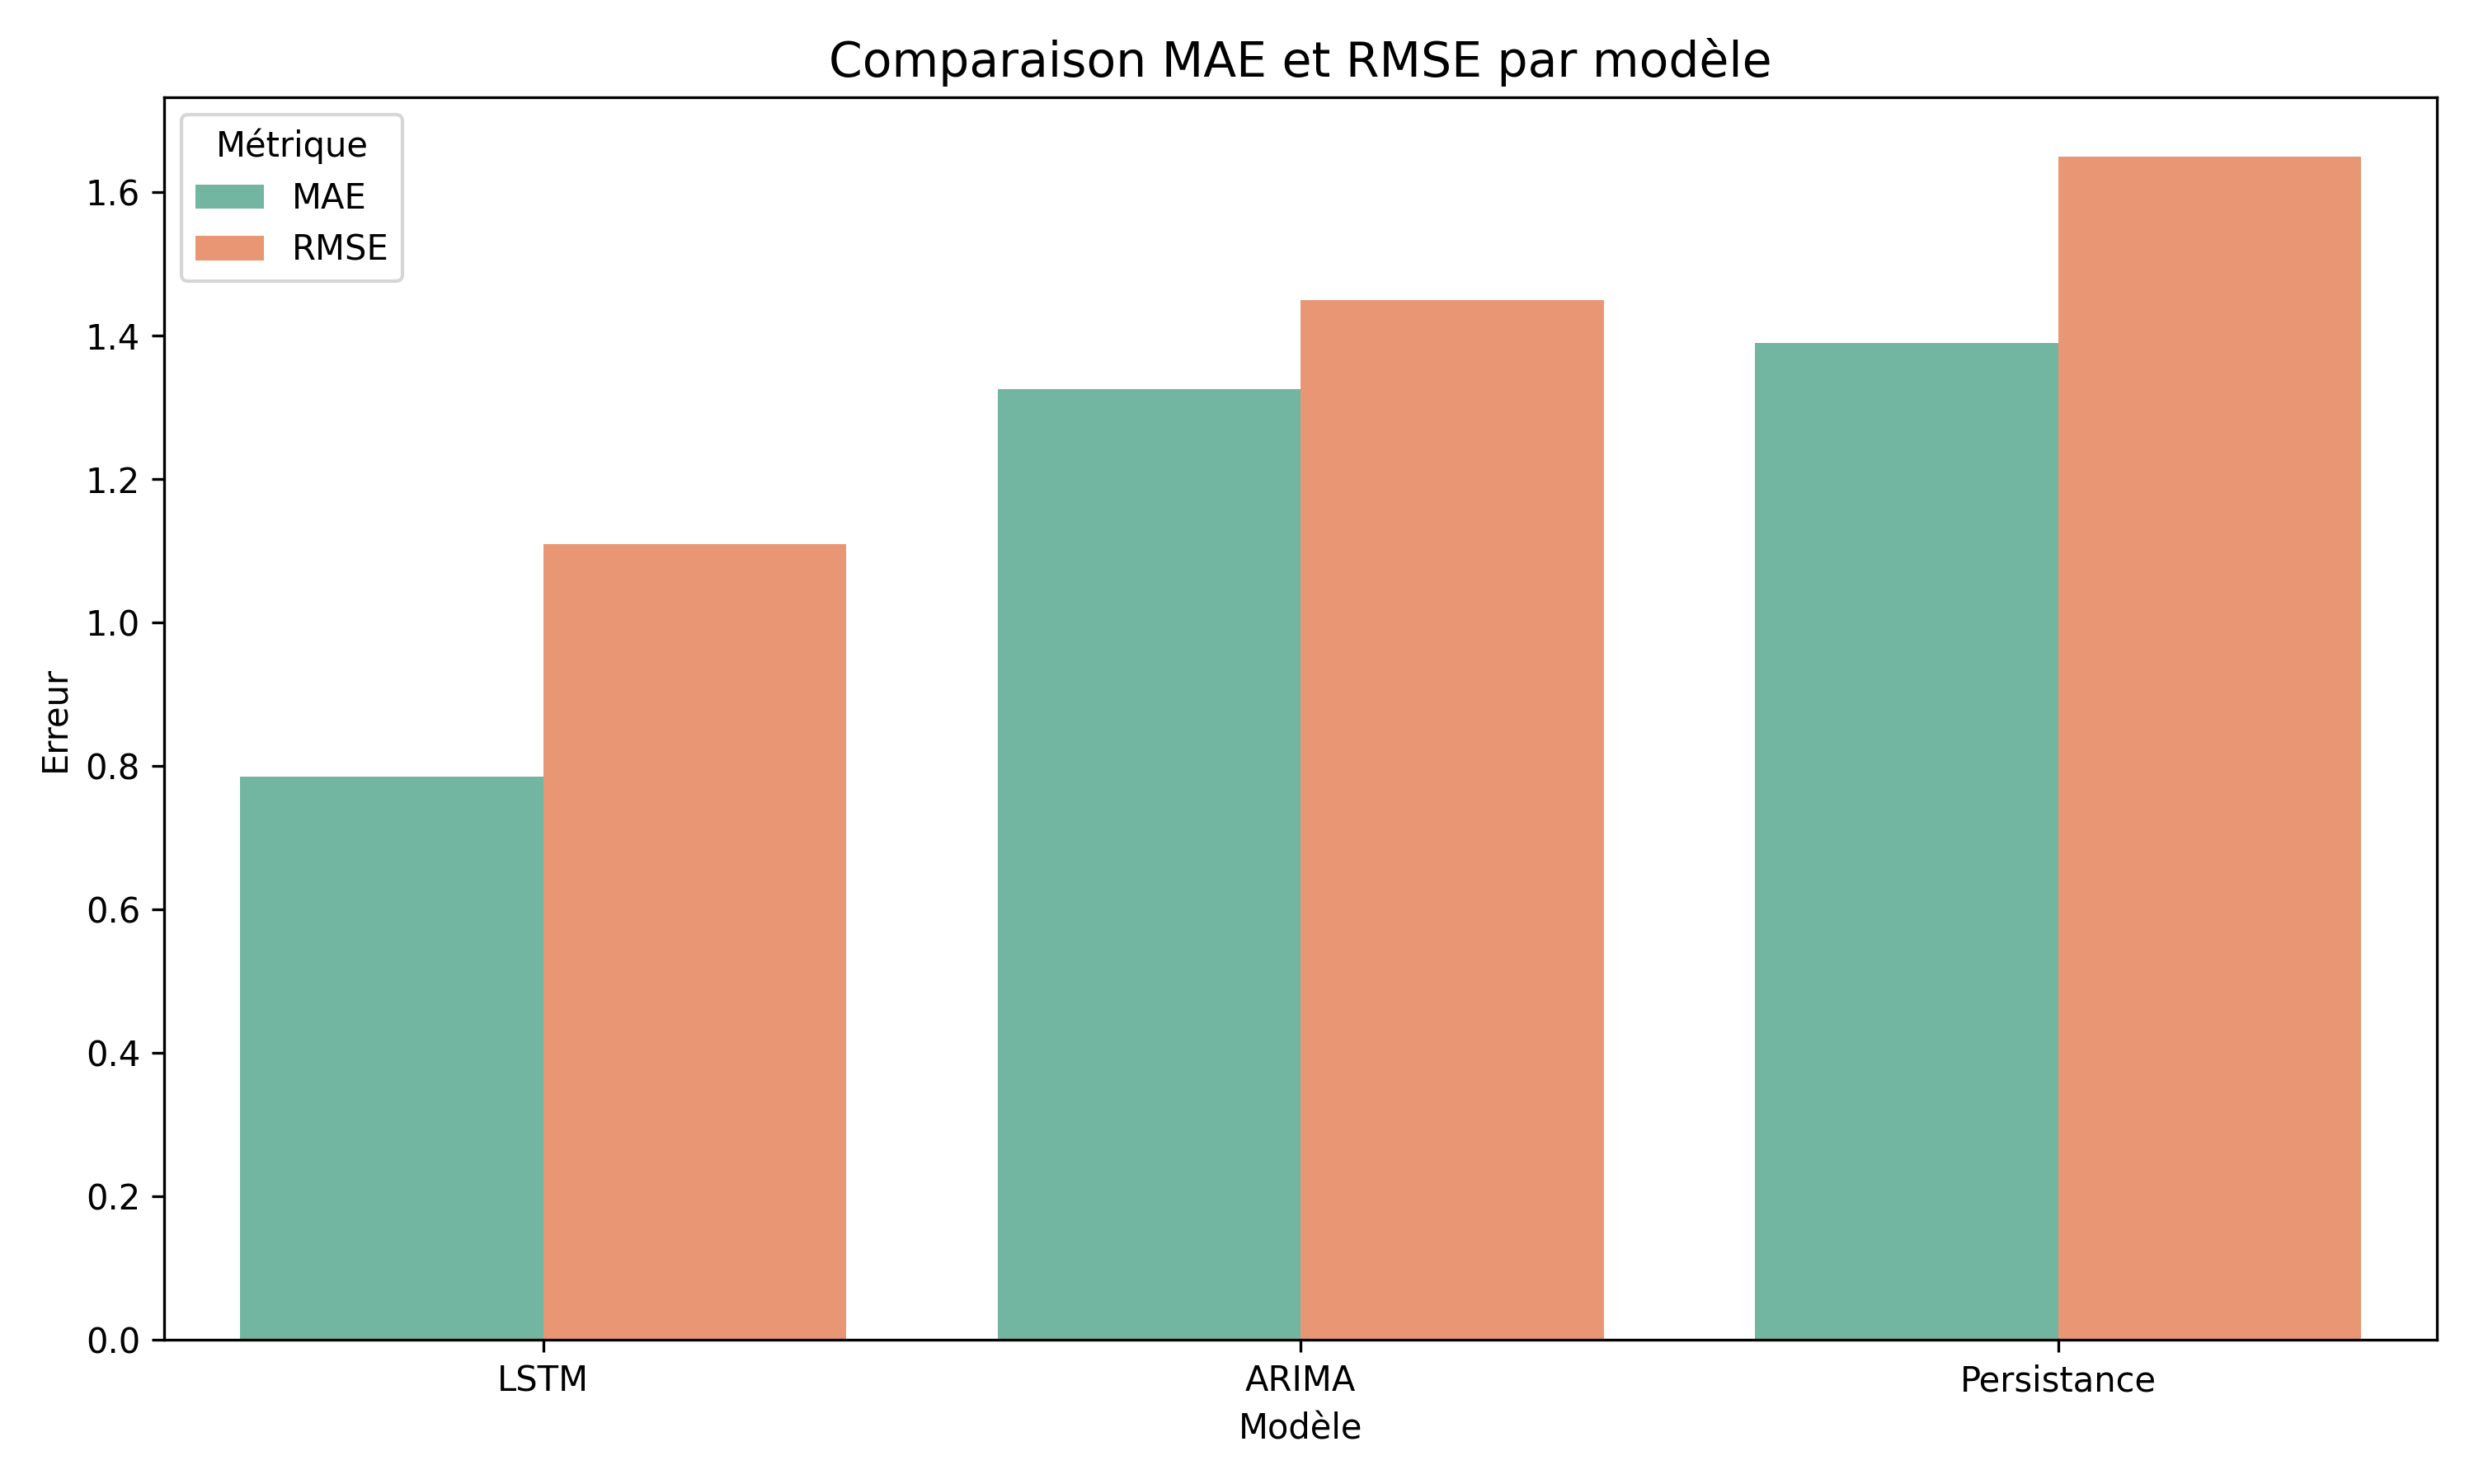
\includegraphics[width=1\textwidth,height=4.6in]{images/comparaison_MAE_RMSE.png}
		    \end{center}
		    \end{minipage}
				
			\caption{Comparaison des métriques\label{Fig 3.6}}
		\end{center}
	\end{figure}%
\section{Résultats de la prévision météoroogique des conditions météorologique au PAD}
	

\subsection{Conception de l’interface web de visualisation}
L’interface utilisateur a été développée avec \textbf{Streamlit}, permettant une visualisation interactive des données météo et marégraphiques. Elle comprend :
\begin{enumerate}
	\item Une carte \textbf{Folium} des stations géolocalisées.
	
	\begin{figure}[H]
		\begin{center}
		 \begin{minipage}{\textwidth}
		 	
		    \begin{center}
		    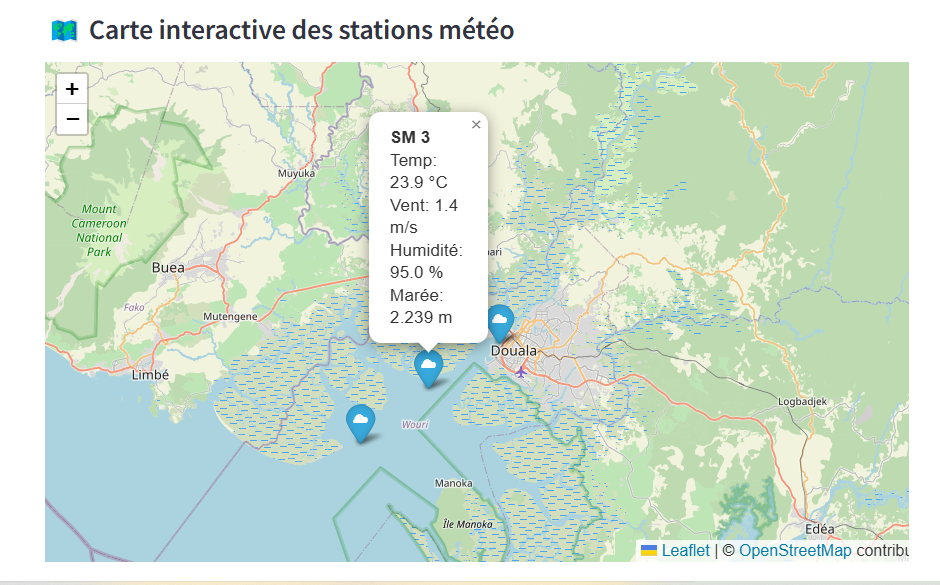
\includegraphics[width=1\textwidth,height=4.6in]{images/SITE_PAD3.png}
		    \caption{visualisation des parametres météorologiques sur chaque station \label{Fig 3.7} }
		    \end{center}
		    \end{minipage}	\\
		    	
			\quad
			
		%	\begin{center}
			\centering
		La Figure \ref{Fig 3.7}  montre l'évolution de chaque paramètres  afin non seulement d'avoir connaissance aux station défectuese et ensuite de faire une comparaison entre les differentes station .
		\item Un accès aux données historiques avec options de filtrage voir Figure \ref{Fig 3.8}.
		\item Une mini-carte \textbf{Windy} embarquée pour la prévision du vent en temps réel cf Figure \ref{Fig 3.10}.
		Un module spécifique est également prévu pour publier chaque matin une prévision automatique de la journée en se basant sur le modèle LSTM et sur des données exogènes (WRF, Copernicus, Windy).
			
		\end{center}
	\end{figure}%	
	\item Des graphiques \textbf{Plotly} pour analyser l’évolution des paramètres par station cf Figure \ref{Fig 3.8}.
	
	\begin{figure}[H]
		\begin{center}
		 \begin{minipage}{\textwidth}
		    \begin{center}
		    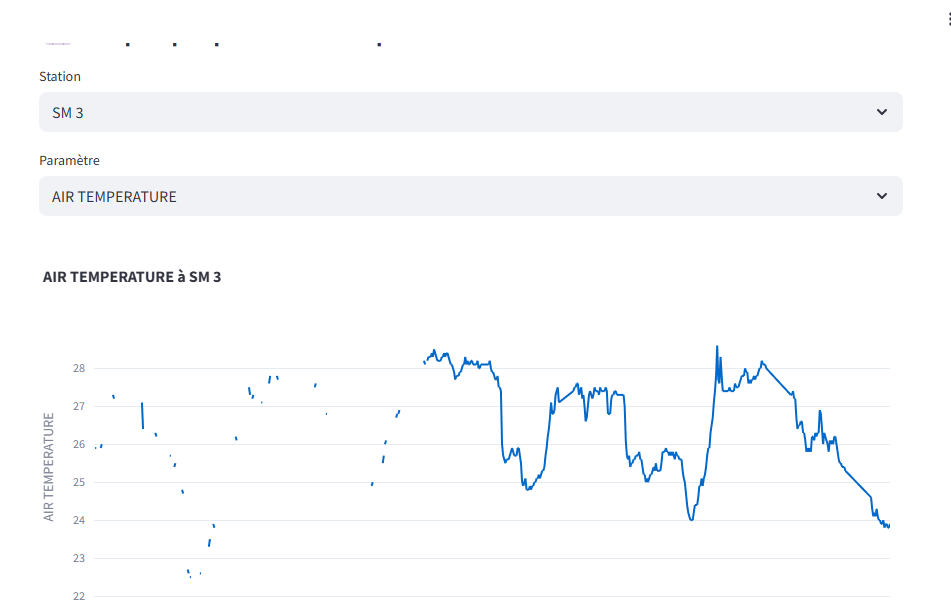
\includegraphics[width=1\textwidth,height=4.6in]{images/SITE_PAD.png}
		    \end{center}
		    \end{minipage}
			\caption{évolution des paramètres par station (pour plus de detail consulter le site \label{Fig 3.8}}
		\end{center}
	\end{figure}%
	

	
	\quad

		\item prevision precipitation et temperature à partir de LSTM et d'autres modèles voir Figure\ref{Fig 3.11}.
	
	\begin{figure}[H]
		\begin{center}
		 \begin{minipage}{\textwidth}
		    \begin{center}
		    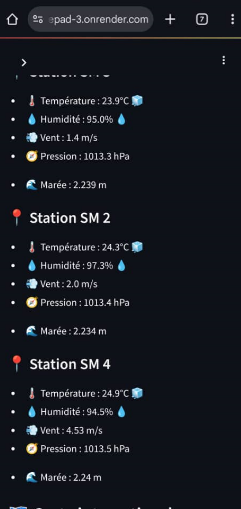
\includegraphics[width=0.6\textwidth]{images/site_pad_donne.png}
		    \end{center}
		    \end{minipage}
		\caption{évolution des paramètres par station (pour plus de detail consulter le site ...\label{Fig 3.9}}
		\end{center}
	\end{figure}%
		\begin{figure}[H]
		\begin{center}
				 \begin{minipage}{\textwidth}
				    \begin{center}
				    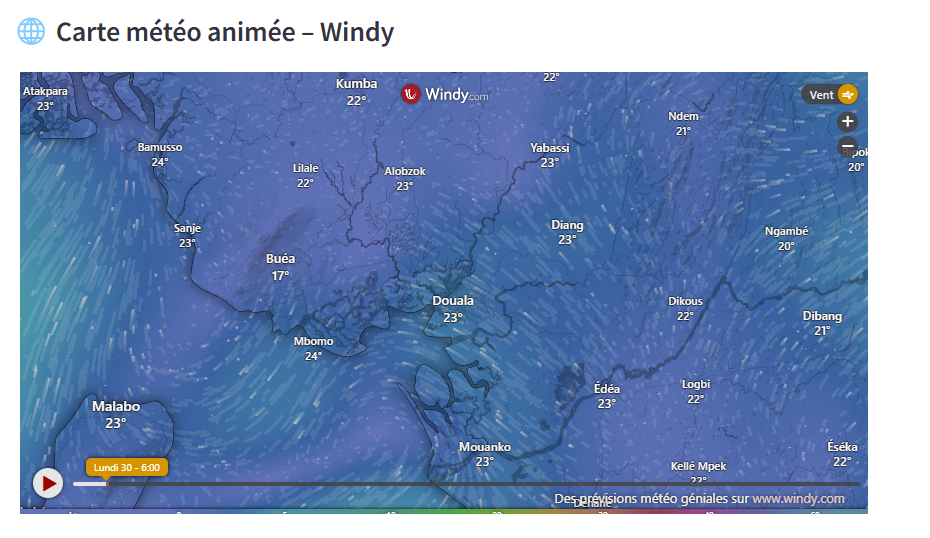
\includegraphics[width=1\textwidth,height=5.6in]{images/site_PAD_windy.png}
				    \end{center}
				    \end{minipage}
				
			\caption{Extrait de Windy pour les previsions  (pour plus de detail consulter le site \label{Fig 3.10}}
		\end{center}
	\end{figure}%
\end{enumerate}



\begin{figure}[H]
	\begin{center}
				 \begin{minipage}{\textwidth}
				    \begin{center}
 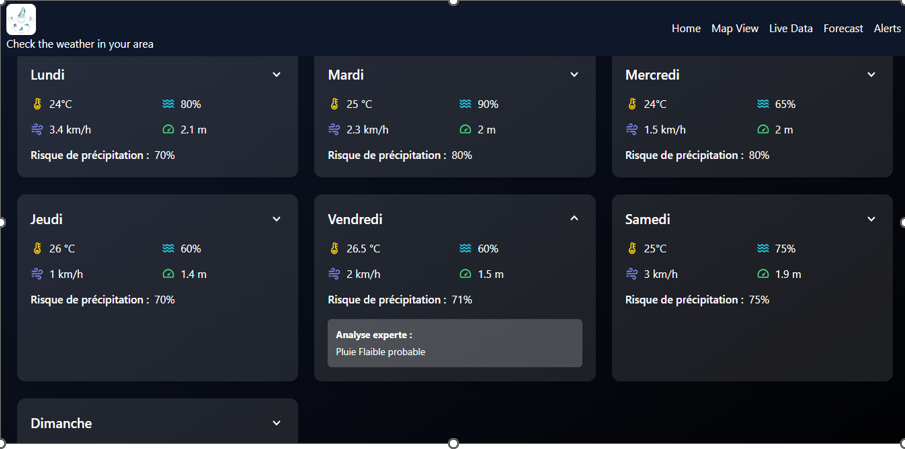
\includegraphics[width=1\textwidth,height=4.6in]{images/prevision_7_jours.png}
				    \end{center}
				    \end{minipage}

			
			\caption{Visualisation de la prevision météorologique du Chenal du Port Autonome de Doual valide du 30/6/25 à 00TU au 06/7/25 à 00TU \label{Fig 
3.11}}.
		\end{center}
\end{figure}%


\section{Intégration et déploiement}

\subsection{Déploiement des données }
\begin{enumerate}
	\item Une API Flask connectée à une base MongoDB Atlas hébergée sur Render, servant les données en temps réel consulter le site por plus information. \\

%	

	
	\subsection{Déploiement des sites web }
	\item Une interface web Streamlit et react  également déployée sur Render (consulter le site por plus information)	
\end{enumerate}
Ce découplage permet une architecture flexible et évolutive, où la base de données et la logique de prédiction peuvent être mises à jour indépendamment de l’interface utilisateur.

\section{Perspectives d’évolution}
Plusieurs améliorations peuvent être envisagées :
\begin{itemize}
	\item Achat d'un super calculateur afin de tourner ces propres modeles .
		\item Instalation d'une connection Ilimitée  et tres fluide.
	\item Automatisation complète du processus de prédiction quotidienne avec envoi des résultats via email ou notification mobile.\\
	\item Amélioration du modèle 
	\item  Renforcement de la sécurité et authentification des accès à l’API.
\end{itemize}

	\section{Application}
	L’application développée permet aux utilisateurs (agents portuaires, pêcheurs, autorités locales) d’accéder à des informations météorologiques et marégraphiques actualisées. Chaque matin, une nouvelle prévision est générée à partir des données récentes et publiée en ligne. La carte interactive et les graphiques permettent une analyse spatio-temporelle des phénomènes.
	Cette solution a été pensée comme un outil de support à la décision, accessible sur le web, et extensible à d’autres régions côtières du Cameroun.
	

\newpage
		\section*{}
	Ce chapitre a présenté la mise en œuvre concrète du système de prévision météo à Douala, depuis l’entraînement du modèle LSTM jusqu’à son intégration dans une application web interactive. Grâce à une architecture modulaire, à une automatisation du flux de données, et à une interface conviviale, cette solution constitue une base fonctionnelle pour la prévision en temps réel. Elle ouvre la voie à une généralisation à d’autres sites et à une intégration progressive de modèles marégraphiques avancés	


%=======================================================================================================================%
\chapter*{ CONCLUSION GÉNÉRALE ET PERSPECTIVES }\addcontentsline{toc}{chapter}{CONCLUSION GÉNÉRALE ET PERSPECTIVES}
\vspace{1cm}
%\chapter{Conclusion Générale et Perspectives}
\label{chap:conclusion}
	
		\quad En somme ,il était question pour nous de développer une solution complète des prévision de état de l'atmosphère  au Port Autonome de Douala  à partir de l’Intelligence Artificielle bien que nous avons utilisé d’autres sources et d’autre  modèle meteorologique comme (Direction Nationale,CAPC-AC,WRF,… ). Ce mémoire a permis de démontrer la faisabilité et l’efficacité d’un système intelligent de prévision des conditions météorologiques pour le Port Autonome de Douala, à partir d’une approche open data et de techniques de machine learning avancées. En combinant des données réelles collectées par des stations installées sur site (SM2, SM3, SM4) avec des modèles LSTM adaptés aux séries temporelles environnementales, nous avons produit des prédictions robustes, exploitables en temps réel.La plateforme web développée constitue une innovation opérationnelle majeure : elle permet non seulement la visualisation en temps réel, mais également la planification intelligente des opérations portuaires, la détection précoce des anomalies et la résilience face aux risques climatiques.
		Bien que certaines limites matérielles et logicielles aient été identifiées (manque de redondance capteur, dépendance à la connectivité Internet, amélioration possible du modèle), les perspectives d’évolution sont prometteuses : extension du système à d’autres ports, intégration de données satellites (NOAA, Copernicus), mise en place de notifications automatiques ou encore hybridation des modèles (LSTM + CNN ou Transformers).Ce projet constitue ainsi une étape décisive vers la modernisation numérique des systèmes de surveillance environnementale portuaire au Cameroun, et s’inscrit dans les ambitions de développement durable, de sécurité maritime et d’innovation technologique
		

		\label{ch:Conclusiongénérale et perspectives} %\thispagestyle{empty}
		\newpage
%	\begin{thebibliography}{99}
	\label{RéférencesBibliographiques}
\markboth{Bibliography}{Bibliography}











%----------------------------------------------------------------------------------------------------------------------------- %






	%\begin{thebibliography}{64}
\begin{thebibliography}{99}
	
	\bibitem{Nicholls2008}
	Nicholls, R. J., et al. (2008).
	\textit{Ranking Port Cities with High Exposure and Vulnerability to Climate Extremes: Exposure Estimates}.
	OECD Environment Working Papers, No. 1. \url{https://doi.org/10.1787/011766488208}
	
	\bibitem{Ngatcha2021}
	Ngatcha Nguiffo, J., Tchindjang, M., \& Nguendo-Yongsi, H. B. (2021).
	\textit{Vulnérabilité des espaces urbains à Douala}.
	Université de Douala.
	
	\bibitem{Bremnes2020}
	Bremnes, J. B. (2020).
	\textit{Ensemble postprocessing using quantile function regression based on quantile forests}.
	Monthly Weather Review, \textbf{148}(1), 403–414. \url{https://doi.org/10.1175/MWR-D-19-0220.1}
	
	\bibitem{Shamshirband2020}
	Shamshirband, S., et al. (2020).
	\textit{A review of artificial intelligence techniques for short-term load forecasting in smart grids}.
	Applied Sciences, \textbf{10}(2), 590. \url{https://doi.org/10.3390/app10020590}
	
	\bibitem{PAD2023}
	Port Autonome de Douala (2023-2024).
	\textit{Rapports techniques et bilans d'activités}. \url{https://meteocameroon.gov.cm}
	
	\bibitem{Doumbia2020}
	Doumbia, M., et al. (2020).
	\textit{Évaluation des coûts économiques de la dégradation de l'environnement : Cas du Grand Abidjan}.
	Banque mondiale. \url{https://documents.worldbank.org/curated/en/985041599010605269}
	
	\bibitem{OMM2023}
	Organisation météorologique mondiale (2023).
	\textit{État des ressources en eau dans le monde 2022}.
	OMM-N°1333. \url{https://library.wmo.int/idurl/4/1333}
	
	\bibitem{Bruckmann2019}
	Bruckmann, L., et al. (2019).
	\textit{Urbanisation, risques naturels et résilience à Douala}.
	EchoGéo, \textbf{48}. \url{https://doi.org/10.4000/echogeo.17483}
	
	\bibitem{PNUE2021}
	PNUE (2021).
	\textit{GEO-6 pour l'Afrique}.
	\url{https://www.unep.org/resources/report/global-environment-outlook-6-africa}
	
	\bibitem{OMM2018}
	OMM (2018).
	\textit{Guide de l’assistance météorologique aux activités maritimes}.
	OMM-N°471. \url{https://library.wmo.int/doc_num.php?explnum_id=5426}
	
	\bibitem{Pena2020}
	Peña, J. M., et al. (2020).
	\textit{Automatic weather stations and GPS integration}.
	Sensors, \textbf{20}(12), 3456. \url{https://doi.org/10.3390/s20123456}
	
	\bibitem{COIUNESCO2016}
	COI-UNESCO (2016).
	\textit{Manuel sur la mesure du niveau de la mer - Volume V}.
	\url{https://unesdoc.unesco.org/ark:/48223/pf0000246981_fre}
	
	\bibitem{Pugh2014}
	Pugh, D. (2014).
	\textit{Sea-Level Science}.
	Cambridge University Press.
	
	\bibitem{Tang2021}
	Tang, L., et al. (2021).
	\textit{Impact of extreme weather on port logistics}.
	Journal of Transport Geography, \textbf{93}, 103045. \url{https://doi.org/10.1016/j.jtrangeo.2021.103045}
	
	\bibitem{Oueslati2019}
	Oueslati, B., et al. (2019).
	\textit{Climate change adaptation in port infrastructure}.
	Transportation Research Part D, \textbf{72}, 289–302. \url{https://doi.org/10.1016/j.trd.2019.05.005}
	
	\bibitem{Lyon2021}
	Lyon, S. W. (2021).
	\textit{Port Risk and Climate Resilience}.
	Water Security, \textbf{12}, 100081.
	
	\bibitem{Bianchi2017}
	Bianchi, F. M., et al. (2017).
	\textit{Echo-state networks dynamics via recurrence}.
	IEEE TNNLS, \textbf{29}(2), 427–439. \url{https://doi.org/10.1109/TNNLS.2017.2663841}
	
	\bibitem{USCG2006}
	USCG \& Alaska DEC. (2006).
	\textit{Incident Report: M/V Cougar Ace listing}.
	Anchorage, Alaska.
	
	\bibitem{Gaillarde2001}
	Gaillarde, C. (2001).
	\textit{Marégraphie et variations du niveau de la mer}.
	SHOM.
	
	\bibitem{GPFMA2024}
	GPFMA. (2024).
	\textit{Gestion portuaire face aux événements marins anormaux}.
	Global Maritime Report.
	
	\bibitem{Murara2018}
	Murara, E. (2018).
	\textit{Hydrography and Port Planning in Africa}.
	Journal of African Ports.
	
	\bibitem{Rotterdam2018}
	Port of Rotterdam \& IBM. (2018).
	\textit{Smart Port Vision: Digital Twin and IoT}.
	Port of Rotterdam Authority.
	
	\bibitem{Martins2019}
	Martins, F. (2019).
	\textit{Ports and Big Data}.
	Maritime Economics \& Logistics.
	
	\bibitem{Russell2020}
	Russell, S., \& Norvig, P. (2020).
	\textit{Artificial Intelligence: A Modern Approach} (4e éd.).
	Pearson.
	
	\bibitem{Mitchell1997}
	Mitchell, T. M. (1997).
	\textit{Machine Learning}.
	McGraw-Hill.
	
	\bibitem{Goodfellow2016}
	Goodfellow, I., et al. (2016).
	\textit{Deep Learning}.
	MIT Press.
	
	\bibitem{LeCun2015}
	LeCun, Y., et al. (2015).
	\textit{Deep Learning}.
	Nature, \textbf{521}(7553), 436–444.
	
	\bibitem{Hyndman2018}
	Hyndman, R. J., \& Athanasopoulos, G. (2018).
	\textit{Forecasting: Principles and Practice}.
	OTexts. \url{https://otexts.com/fpp3/}
	
	\bibitem{Zhang2020}
	Zhang, G., et al. (2020).
	\textit{Forecasting with artificial neural networks}.
	International Journal of Forecasting, \textbf{36}(1), 1–35. \url{https://doi.org/10.1016/j.ijforecast.2019.05.001}
	
	\bibitem{Kiranyaz2015}
	Kiranyaz, S., et al. (2015).
	\textit{Real-time prediction using 1D CNNs}.
	IEEE Transactions.
	
	\bibitem{Yu2022}
	Yu, M., et al. (2022).
	\textit{Short-term weather prediction using 1D-CNN}.
	Environmental Modelling \& Software, \textbf{150}, 105343. \url{https://doi.org/10.1016/j.envsoft.2022.105343}
	
	\bibitem{Graves2005}
	Graves, A., \& Schmidhuber, J. (2005).
	\textit{Framewise phoneme classification with bidirectional LSTM}.
	ICANN.
	
	\bibitem{Zhang2021}
	Zhang, Y., et al. (2021).
	\textit{Multivariate weather time series forecasting}.
	Atmosphere, \textbf{12}(3), 356. \url{https://doi.org/10.3390/atmos12030356}
	
	\bibitem{Hochreiter1997}
	Hochreiter, S., \& Schmidhuber, J. (1997).
	\textit{Long Short-Term Memory}.
	Neural Computation, \textbf{9}(8), 1735–1780.
	
	\bibitem{Wang2021}
	Wang, B., et al. (2021).
	\textit{Storm surge prediction using CNN-LSTM}.
	Acta Oceanologica Sinica, \textbf{40}, 104–118. \url{https://doi.org/10.1007/s13131-021-1763-9}
	
	\bibitem{Fernandes2020}
	Fernandes, S. O., et al. (2020).
	\textit{Forecasting ocean parameters with deep learning}.
	Marine Systems, \textbf{203}, 103263.
	
	\bibitem{Zhou2022}
	Zhou, J., et al. (2022).
	\textit{Prévision de débits fluviaux à l'aide de modèles hybrides}.
	Université Paris-Saclay.
	
	\bibitem{Akinsanola2015}
	Akinsanola, A. A., \& Ogunjobi, K. O. (2015).
	\textit{Rainfall and temperature variability over Nigeria}.
	Theoretical and Applied Climatology, \textbf{123}, 369–384. \url{https://doi.org/10.1007/s00704-014-1350-7}
	
	\bibitem{Abraham2019}
	Abraham, A., et al. (2019).
	\textit{Postprocessing WRF outputs using ML}.
	Atmospheric Research, \textbf{228}, 123–135.
	
	\bibitem{Shi2015}
	Shi, X., et al. (2015).
	\textit{Convolutional LSTM network for precipitation nowcasting}.
	NIPS.
	
	\bibitem{UNDRR2022}
	UNDRR (2022).
	\textit{Alerte précoce et action rapide pour tous}.
	\url{https://iddrr.undrr.org/media}
	
	\bibitem{Chalapathy2019}
	Chalapathy, R., \& Chawla, S. (2019).
	\textit{Deep Learning for Anomaly Detection: A Survey}.
	arXiv:1901.03407. \url{https://doi.org/10.48550/arXiv.1901.03407}
	
	\bibitem{Kitchin2014}
	Kitchin, R. (2014).
	\textit{The Data Revolution}.
	Sage.
	
	\bibitem{OMM2021}
	OMM (2021).
	\textit{État du climat mondial 2021}.
	\url{https://library.wmo.int/viewer/54009/download}
	
	\bibitem{UNECA2020}
	UNECA (2020).
	\textit{Open Data for Africa}.
	\url{https://uneca.org}
	
	\bibitem{Morozov2019}
	Morozov, E. (2019).
	\textit{Cartographie 4.0}.
	Responsabilité \& Environnement, n°94.
	
	\bibitem{Janssen2012}
	Janssen, M., et al. (2012).
	\textit{Benefits, adoption barriers and myths of open data}.
	Government Information Quarterly, \textbf{29}(4), 512–520.
	
	\bibitem{EuropeanCommission2019}
	European Commission. (2019).
	\textit{Copernicus Work Programme}.
	\url{https://www.copernicus.eu}
	
	\bibitem{Madianou2019}
	Madianou, M. (2019).
	\textit{Technocolonialism: Digital innovation and data in humanitarian response}.
	Social Media + Society.
	
	\bibitem{Greff2017}
	Greff, K., et al. (2017).
	\textit{LSTM: A Search Space Odyssey}.
	IEEE Transactions on Neural Networks and Learning Systems, \textbf{28}(10), 2222–2232.
	
\end{thebibliography}


	

	
	

%	
% %###################### Annexes ####################### #######################################################
 
    \clearpage
    \phantomsection
    \chapter*{Annexes}
    
    	\centering
 \textbf{1-TideMasterExpress.pdf}\\	
 \textbf{2-Lien vers le dépôt GitHub du projet}
  
  Le code source complet, la source  de données ainsi que les scripts,l'ensemble des graphes et document utilisé; d'entraînement et de visualisation sont disponibles sur GitHub à l'adresse suivante :
  
  \href{https://github.com/Thierry-Engoulou/projet_fin_d_etude}{https://github.com/Thierry-Engoulou/projet\_fin\_d\_etude}
  
	\bibliographystyle{plain}
	\bibliography{ref_grobner}
	
\end{document}
